% !TEX output_directory=output
\documentclass{beamer}

\usepackage[beamer]{../wjk}
\usepackage[font=footnotesize]{caption}

% uncomment to only show notes in PDF
% \setbeameroption{show only notes}

\bibliography{../refs.bib}
\graphicspath{{../graphics/}}

\title[RL for Quantum Control in NMR]{Using Reinforcement Learning for Quantum Control in Magnetic Resonance}
\author[Will Kaufman]{
Will Kaufman\inst{1}
% \and Benjamin Alford\inst{1}
% \and Pai Peng\inst{2} \\
% \and Xiaoyang Huang\inst{2}
% \and Linta Joseph\inst{1}
% \and Paola Cappellaro\inst{2}
% \and Chandrasekhar Ramanathan\inst{1}
}
\date[Spring 2021]{May 24, 2021 \\
% {\footnotesize NSF support under Grants OIA-1921199, PHY1734011, and PHY1915218.}
}
\institute[Dartmouth College]{
\inst{1}Department of Physics and Astronomy, Dartmouth College \\
Hanover, NH 03755, USA
% \and
% \inst{2}Research Laboratory of Electronics, Massachusetts Institute of Technology \\
% Cambridge, Massachusetts 02139, USA
}

\vfill

\titlegraphic{
\includegraphics[height=.06\textheight]{qisD.png}
\hfill
\includegraphics[height=.06\textheight]{Dartmouth.pdf}
% \hfill
% \includegraphics[height=.06\textheight]{mit_logo.png}
}

\begin{document}

\frame{\titlepage}

% \begin{frame}
% \frametitle{Table of Contents}
% \tableofcontents
% \end{frame}

\section{Spin systems}


\begin{frame}{NMR and spin systems}

\begin{figure}
\centering
\scalebox{.7}{


\tikzset{every picture/.style={line width=0.75pt}} %set default line width to 0.75pt        

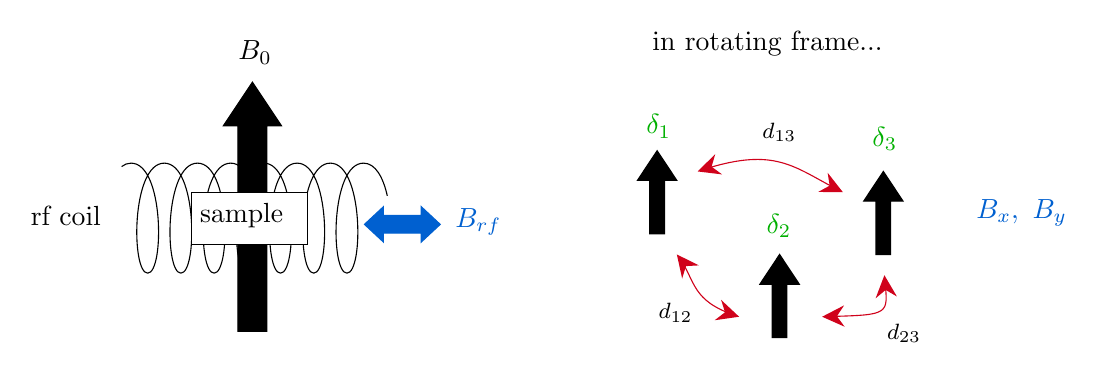
\begin{tikzpicture}[x=0.75pt,y=0.75pt,yscale=-1,xscale=1]
%uncomment if require: \path (0,300); %set diagram left start at 0, and has height of 300

%Shape: Spring [id:dp2646957379333682] 
\draw   (60.5,127.65) .. controls (61.84,126.59) and (63.36,126) .. (65.05,126) .. controls (81.05,126) and (81.05,179) .. (73.05,179) .. controls (65.05,179) and (65.05,126) .. (81.05,126) .. controls (97.05,126) and (97.05,179) .. (89.05,179) .. controls (81.05,179) and (81.05,126) .. (97.05,126) .. controls (113.05,126) and (113.05,179) .. (105.05,179) .. controls (97.05,179) and (97.05,126) .. (113.05,126) .. controls (129.05,126) and (129.05,179) .. (121.05,179) .. controls (113.05,179) and (113.05,126) .. (129.05,126) .. controls (145.05,126) and (145.05,179) .. (137.05,179) .. controls (129.05,179) and (129.05,126) .. (145.05,126) .. controls (161.05,126) and (161.05,179) .. (153.05,179) .. controls (145.05,179) and (145.05,126) .. (161.05,126) .. controls (177.05,126) and (177.05,179) .. (169.05,179) .. controls (161.05,179) and (161.05,126) .. (177.05,126) .. controls (182.83,126) and (186.52,132.91) .. (188.5,141.74) ;
%Up Arrow [id:dp6494976910138215] 
\draw  [fill={rgb, 255:red, 0; green, 0; blue, 0 }  ,fill opacity=1 ] (109.5,108) -- (123.5,87) -- (137.5,108) -- (130.5,108) -- (130.5,207) -- (116.5,207) -- (116.5,108) -- cycle ;
%Left Right Arrow [id:dp373669277385548] 
\draw  [color={rgb, 255:red, 0; green, 96; blue, 208 }  ,draw opacity=1 ][fill={rgb, 255:red, 0; green, 96; blue, 208 }  ,fill opacity=1 ] (177.5,155.5) -- (186.63,147) -- (186.63,151.25) -- (204.88,151.25) -- (204.88,147) -- (214,155.5) -- (204.88,164) -- (204.88,159.75) -- (186.63,159.75) -- (186.63,164) -- cycle ;
%Up Arrow [id:dp5658158221948956] 
\draw  [fill={rgb, 255:red, 0; green, 0; blue, 0 }  ,fill opacity=1 ] (309,134.33) -- (318.5,120) -- (328,134.33) -- (322.03,134.33) -- (322.03,160) -- (314.97,160) -- (314.97,134.33) -- cycle ;
%Up Arrow [id:dp6557849832321283] 
\draw  [fill={rgb, 255:red, 0; green, 0; blue, 0 }  ,fill opacity=1 ] (368,184.33) -- (377.5,170) -- (387,184.33) -- (381.03,184.33) -- (381.03,210) -- (373.97,210) -- (373.97,184.33) -- cycle ;
%Up Arrow [id:dp7240484081648103] 
\draw  [fill={rgb, 255:red, 0; green, 0; blue, 0 }  ,fill opacity=1 ] (418,144.33) -- (427.5,130) -- (437,144.33) -- (431.03,144.33) -- (431.03,170) -- (423.97,170) -- (423.97,144.33) -- cycle ;
%Curve Lines [id:da475332234824406] 
\draw [color={rgb, 255:red, 208; green, 2; blue, 27 }  ,draw opacity=1 ]   (329.84,172.56) .. controls (336.95,183.28) and (335.51,192.13) .. (355.4,199.13) ;
\draw [shift={(358,200)}, rotate = 197.49] [fill={rgb, 255:red, 208; green, 2; blue, 27 }  ,fill opacity=1 ][line width=0.08]  [draw opacity=0] (10.72,-5.15) -- (0,0) -- (10.72,5.15) -- (7.12,0) -- cycle    ;
\draw [shift={(328,170)}, rotate = 51.91] [fill={rgb, 255:red, 208; green, 2; blue, 27 }  ,fill opacity=1 ][line width=0.08]  [draw opacity=0] (10.72,-5.15) -- (0,0) -- (10.72,5.15) -- (7.12,0) -- cycle    ;
%Curve Lines [id:da5359587773784383] 
\draw [color={rgb, 255:red, 208; green, 2; blue, 27 }  ,draw opacity=1 ]   (401.47,199.9) .. controls (430.46,199.07) and (429.79,198.99) .. (428.27,182.96) ;
\draw [shift={(428,180)}, rotate = 445.16] [fill={rgb, 255:red, 208; green, 2; blue, 27 }  ,fill opacity=1 ][line width=0.08]  [draw opacity=0] (10.72,-5.15) -- (0,0) -- (10.72,5.15) -- (7.12,0) -- cycle    ;
\draw [shift={(398,200)}, rotate = 358.33] [fill={rgb, 255:red, 208; green, 2; blue, 27 }  ,fill opacity=1 ][line width=0.08]  [draw opacity=0] (10.72,-5.15) -- (0,0) -- (10.72,5.15) -- (7.12,0) -- cycle    ;
%Curve Lines [id:da3330816205973127] 
\draw [color={rgb, 255:red, 208; green, 2; blue, 27 }  ,draw opacity=1 ]   (341.37,128.9) .. controls (375.59,118.07) and (384.43,127.94) .. (405.64,138.81) ;
\draw [shift={(408,140)}, rotate = 206.24] [fill={rgb, 255:red, 208; green, 2; blue, 27 }  ,fill opacity=1 ][line width=0.08]  [draw opacity=0] (10.72,-5.15) -- (0,0) -- (10.72,5.15) -- (7.12,0) -- cycle    ;
\draw [shift={(338,130)}, rotate = 341.27] [fill={rgb, 255:red, 208; green, 2; blue, 27 }  ,fill opacity=1 ][line width=0.08]  [draw opacity=0] (10.72,-5.15) -- (0,0) -- (10.72,5.15) -- (7.12,0) -- cycle    ;

% Text Node
\draw  [fill={rgb, 255:red, 255; green, 255; blue, 255 }  ,fill opacity=1 ]  (94,140) -- (150,140) -- (150,165) -- (94,165) -- cycle  ;
\draw (97,144) node [anchor=north west][inner sep=0.75pt]   [align=left] {sample};
% Text Node
\draw (115.5,65.9) node [anchor=north west][inner sep=0.75pt]    {$B_{0}$};
% Text Node
\draw (15.5,145.5) node [anchor=north west][inner sep=0.75pt]   [align=left] {rf coil};
% Text Node
\draw (220,146.4) node [anchor=north west][inner sep=0.75pt]  [color={rgb, 255:red, 0; green, 96; blue, 208 }  ,opacity=1 ]  {$B_{\text{rf}}$};
% Text Node
\draw (318,192.4) node [anchor=north west][inner sep=0.75pt]  [font=\footnotesize]  {$d_{12}$};
% Text Node
\draw (428,202.4) node [anchor=north west][inner sep=0.75pt]  [font=\footnotesize]  {$d_{23}$};
% Text Node
\draw (368,105.4) node [anchor=north west][inner sep=0.75pt]  [font=\footnotesize]  {$d_{13}$};
% Text Node
\draw (312,101.4) node [anchor=north west][inner sep=0.75pt]  [color={rgb, 255:red, 0; green, 176; blue, 0 }  ,opacity=1 ]  {$\delta _{1}$};
% Text Node
\draw (370,149.4) node [anchor=north west][inner sep=0.75pt]  [color={rgb, 255:red, 0; green, 176; blue, 0 }  ,opacity=1 ]  {$\delta _{2}$};
% Text Node
\draw (421,107.4) node [anchor=north west][inner sep=0.75pt]  [color={rgb, 255:red, 0; green, 176; blue, 0 }  ,opacity=1 ]  {$\delta _{3}$};
% Text Node
\draw (315,61) node [anchor=north west][inner sep=0.75pt]   [align=left] {in rotating frame...};
% Text Node
\draw (471,142.4) node [anchor=north west][inner sep=0.75pt]  [color={rgb, 255:red, 0; green, 96; blue, 208 }  ,opacity=1 ]  {$B_{\text{x}} ,\ B_{y}$};


\end{tikzpicture}

}
\end{figure}

% \begin{figure}
% \centering
% 

\tikzset{every picture/.style={line width=0.75pt}} %set default line width to 0.75pt

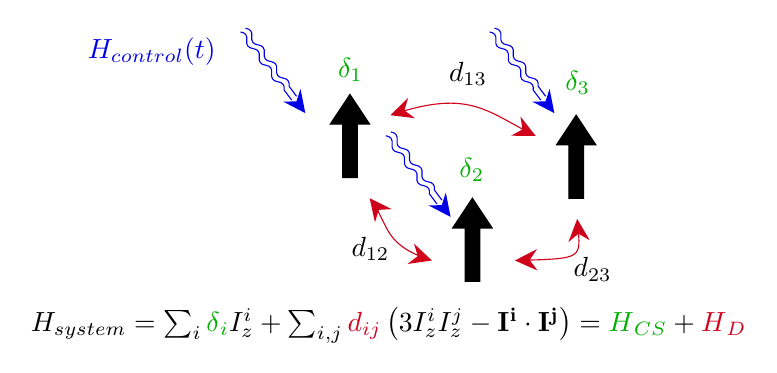
\begin{tikzpicture}[x=0.75pt,y=0.75pt,yscale=-1,xscale=1]
%uncomment if require: \path (0,321); %set diagram left start at 0, and has height of 321

%Up Arrow [id:dp3616533286619681]
\draw  [fill={rgb, 255:red, 0; green, 0; blue, 0 }  ,fill opacity=1 ] (156,55.33) -- (165.5,41) -- (175,55.33) -- (169.03,55.33) -- (169.03,81) -- (161.97,81) -- (161.97,55.33) -- cycle ;
%Up Arrow [id:dp5012912754811447]
\draw  [fill={rgb, 255:red, 0; green, 0; blue, 0 }  ,fill opacity=1 ] (215,105.33) -- (224.5,91) -- (234,105.33) -- (228.03,105.33) -- (228.03,131) -- (220.97,131) -- (220.97,105.33) -- cycle ;
%Up Arrow [id:dp52188591349806]
\draw  [fill={rgb, 255:red, 0; green, 0; blue, 0 }  ,fill opacity=1 ] (265,65.33) -- (274.5,51) -- (284,65.33) -- (278.03,65.33) -- (278.03,91) -- (270.97,91) -- (270.97,65.33) -- cycle ;
%Curve Lines [id:da4574392367290909]
\draw [color={rgb, 255:red, 208; green, 2; blue, 27 }  ,draw opacity=1 ]   (176.84,93.56) .. controls (183.95,104.28) and (182.51,113.13) .. (202.4,120.13) ;
\draw [shift={(205,121)}, rotate = 197.49] [fill={rgb, 255:red, 208; green, 2; blue, 27 }  ,fill opacity=1 ][line width=0.08]  [draw opacity=0] (10.72,-5.15) -- (0,0) -- (10.72,5.15) -- (7.12,0) -- cycle    ;
\draw [shift={(175,91)}, rotate = 51.91] [fill={rgb, 255:red, 208; green, 2; blue, 27 }  ,fill opacity=1 ][line width=0.08]  [draw opacity=0] (10.72,-5.15) -- (0,0) -- (10.72,5.15) -- (7.12,0) -- cycle    ;
%Curve Lines [id:da7885055809075856]
\draw [color={rgb, 255:red, 208; green, 2; blue, 27 }  ,draw opacity=1 ]   (248.47,120.9) .. controls (277.46,120.07) and (276.79,119.99) .. (275.27,103.96) ;
\draw [shift={(275,101)}, rotate = 445.16] [fill={rgb, 255:red, 208; green, 2; blue, 27 }  ,fill opacity=1 ][line width=0.08]  [draw opacity=0] (10.72,-5.15) -- (0,0) -- (10.72,5.15) -- (7.12,0) -- cycle    ;
\draw [shift={(245,121)}, rotate = 358.33] [fill={rgb, 255:red, 208; green, 2; blue, 27 }  ,fill opacity=1 ][line width=0.08]  [draw opacity=0] (10.72,-5.15) -- (0,0) -- (10.72,5.15) -- (7.12,0) -- cycle    ;
%Curve Lines [id:da5782733153480035]
\draw [color={rgb, 255:red, 208; green, 2; blue, 27 }  ,draw opacity=1 ]   (188.37,49.9) .. controls (222.59,39.07) and (231.43,48.94) .. (252.64,59.81) ;
\draw [shift={(255,61)}, rotate = 206.24] [fill={rgb, 255:red, 208; green, 2; blue, 27 }  ,fill opacity=1 ][line width=0.08]  [draw opacity=0] (10.72,-5.15) -- (0,0) -- (10.72,5.15) -- (7.12,0) -- cycle    ;
\draw [shift={(185,51)}, rotate = 341.27] [fill={rgb, 255:red, 208; green, 2; blue, 27 }  ,fill opacity=1 ][line width=0.08]  [draw opacity=0] (10.72,-5.15) -- (0,0) -- (10.72,5.15) -- (7.12,0) -- cycle    ;

%Straight Lines [id:da5939121577594202]
\draw [color={rgb, 255:red, 0; green, 0; blue, 231 }  ,draw opacity=1 ]   (115.2,9.1) .. controls (117.53,9.43) and (118.53,10.77) .. (118.2,13.1) .. controls (117.87,15.43) and (118.87,16.77) .. (121.2,17.1) .. controls (123.53,17.43) and (124.53,18.77) .. (124.2,21.1) .. controls (123.87,23.43) and (124.87,24.77) .. (127.2,25.1) .. controls (129.53,25.43) and (130.53,26.77) .. (130.2,29.1) .. controls (129.87,31.43) and (130.87,32.77) .. (133.2,33.1) .. controls (135.53,33.43) and (136.53,34.77) .. (136.2,37.1) -- (138,39.5) -- (139.8,41.9)(112.8,10.9) .. controls (115.13,11.23) and (116.13,12.57) .. (115.8,14.9) .. controls (115.47,17.23) and (116.47,18.57) .. (118.8,18.9) .. controls (121.13,19.23) and (122.13,20.57) .. (121.8,22.9) .. controls (121.47,25.23) and (122.47,26.57) .. (124.8,26.9) .. controls (127.13,27.23) and (128.13,28.57) .. (127.8,30.9) .. controls (127.47,33.23) and (128.47,34.57) .. (130.8,34.9) .. controls (133.13,35.23) and (134.13,36.57) .. (133.8,38.9) -- (135.6,41.3) -- (137.4,43.7) ;
\draw [shift={(144,50)}, rotate = 233.13] [fill={rgb, 255:red, 0; green, 0; blue, 231 }  ,fill opacity=1 ][line width=0.08]  [draw opacity=0] (10.72,-5.15) -- (0,0) -- (10.72,5.15) -- (7.12,0) -- cycle    ;
%Straight Lines [id:da5935560230770542]
\draw [color={rgb, 255:red, 0; green, 0; blue, 231 }  ,draw opacity=1 ]   (235.2,9.1) .. controls (237.53,9.43) and (238.53,10.77) .. (238.2,13.1) .. controls (237.87,15.43) and (238.87,16.77) .. (241.2,17.1) .. controls (243.53,17.43) and (244.53,18.77) .. (244.2,21.1) .. controls (243.87,23.43) and (244.87,24.77) .. (247.2,25.1) .. controls (249.53,25.43) and (250.53,26.77) .. (250.2,29.1) .. controls (249.87,31.43) and (250.87,32.77) .. (253.2,33.1) .. controls (255.53,33.43) and (256.53,34.77) .. (256.2,37.1) -- (258,39.5) -- (259.8,41.9)(232.8,10.9) .. controls (235.13,11.23) and (236.13,12.57) .. (235.8,14.9) .. controls (235.47,17.23) and (236.47,18.57) .. (238.8,18.9) .. controls (241.13,19.23) and (242.13,20.57) .. (241.8,22.9) .. controls (241.47,25.23) and (242.47,26.57) .. (244.8,26.9) .. controls (247.13,27.23) and (248.13,28.57) .. (247.8,30.9) .. controls (247.47,33.23) and (248.47,34.57) .. (250.8,34.9) .. controls (253.13,35.23) and (254.13,36.57) .. (253.8,38.9) -- (255.6,41.3) -- (257.4,43.7) ;
\draw [shift={(264,50)}, rotate = 233.13] [fill={rgb, 255:red, 0; green, 0; blue, 231 }  ,fill opacity=1 ][line width=0.08]  [draw opacity=0] (10.72,-5.15) -- (0,0) -- (10.72,5.15) -- (7.12,0) -- cycle    ;
%Straight Lines [id:da7272100103209711]
\draw [color={rgb, 255:red, 0; green, 0; blue, 231 }  ,draw opacity=1 ]   (185.2,59.1) .. controls (187.53,59.43) and (188.53,60.77) .. (188.2,63.1) .. controls (187.87,65.43) and (188.87,66.77) .. (191.2,67.1) .. controls (193.53,67.43) and (194.53,68.77) .. (194.2,71.1) .. controls (193.87,73.43) and (194.87,74.77) .. (197.2,75.1) .. controls (199.53,75.43) and (200.53,76.77) .. (200.2,79.1) .. controls (199.87,81.43) and (200.87,82.77) .. (203.2,83.1) .. controls (205.53,83.43) and (206.53,84.77) .. (206.2,87.1) -- (208,89.5) -- (209.8,91.9)(182.8,60.9) .. controls (185.13,61.23) and (186.13,62.57) .. (185.8,64.9) .. controls (185.47,67.23) and (186.47,68.57) .. (188.8,68.9) .. controls (191.13,69.23) and (192.13,70.57) .. (191.8,72.9) .. controls (191.47,75.23) and (192.47,76.57) .. (194.8,76.9) .. controls (197.13,77.23) and (198.13,78.57) .. (197.8,80.9) .. controls (197.47,83.23) and (198.47,84.57) .. (200.8,84.9) .. controls (203.13,85.23) and (204.13,86.57) .. (203.8,88.9) -- (205.6,91.3) -- (207.4,93.7) ;
\draw [shift={(214,100)}, rotate = 233.13] [fill={rgb, 255:red, 0; green, 0; blue, 231 }  ,fill opacity=1 ][line width=0.08]  [draw opacity=0] (10.72,-5.15) -- (0,0) -- (10.72,5.15) -- (7.12,0) -- cycle    ;


% Text Node
\draw (10.5,142.4) node [anchor=north west][inner sep=0.75pt]    {$H_{\text{system}} =\sum _{i}\textcolor[rgb]{0,0.69,0}{\delta }\textcolor[rgb]{0,0.69,0}{_{i}} I^{i}_{z} +\sum _{i,j}\textcolor[rgb]{0.82,0.01,0.11}{d}\textcolor[rgb]{0.82,0.01,0.11}{_{ij}}\left( 3I^{i}_{z} I^{j}_{z} -\mathbf{I^{i}} \cdot \mathbf{I^{j}}\right) =\textcolor[rgb]{0,0.69,0}{H}\textcolor[rgb]{0,0.69,0}{_{\text{CS}}} +\textcolor[rgb]{0.82,0.01,0.11}{H}\textcolor[rgb]{0.82,0.01,0.11}{_{D}}$};
% Text Node
\draw (165,108.4) node [anchor=north west][inner sep=0.75pt]  [font=\normalsize]  {$d_{12}$};
% Text Node
\draw (272,118.4) node [anchor=north west][inner sep=0.75pt]  [font=\normalsize]  {$d_{23}$};
% Text Node
\draw (212,24.4) node [anchor=north west][inner sep=0.75pt]  [font=\normalsize]  {$d_{13}$};
% Text Node
\draw (158.5,22.4) node [anchor=north west][inner sep=0.75pt]  [color={rgb, 255:red, 0; green, 175; blue, 0 }  ,opacity=1 ]  {$\delta _{1}$};
% Text Node
\draw (217,70.4) node [anchor=north west][inner sep=0.75pt]  [color={rgb, 255:red, 0; green, 175; blue, 0 }  ,opacity=1 ]  {$\delta _{2}$};
% Text Node
\draw (268,28.4) node [anchor=north west][inner sep=0.75pt]  [color={rgb, 255:red, 0; green, 175; blue, 0 }  ,opacity=1 ]  {$\delta _{3}$};
% Text Node
\draw (38,12.4) node [anchor=north west][inner sep=0.75pt]  [color={rgb, 255:red, 0; green, 0; blue, 231 }  ,opacity=1 ]  {$H_{\text{control}}( t)$};


\end{tikzpicture}

% \end{figure}

\[
H_{\text{sys}} =\sum _{i}\textcolor[rgb]{0,0.69,0}{\delta_{i}} I^{i}_{z}
    + \sum _{i,j}\textcolor[rgb]{0.82,0.01,0.11}{d_{ij}}\left( 3I^{i}_{z} I^{j}_{z} -\mathbf{I^{i}} \cdot \mathbf{I^{j}}\right)
    = \textcolor[rgb]{0,0.69,0}{H_{\text{CS}}}
    + \textcolor[rgb]{0.82,0.01,0.11}{H_{D}}
\]


\note{
Only focusing on closed system dynamics with global control (spins are not addressed individually).
}

\end{frame}


\begin{frame}{Quantum control in spin systems}

\[
    H_{\text{ctrl}}(t) = -B_x(t) \sum_i \gamma_n^i I_x^i -B_y(t) \sum_i \gamma_n^i I_y^i
\]

Can apply \textbf{$\pi/2$-pulses} that collectively rotate spins

\begin{figure}
    \centering
    \scalebox{.5}{
    

\tikzset{every picture/.style={line width=0.75pt}} %set default line width to 0.75pt

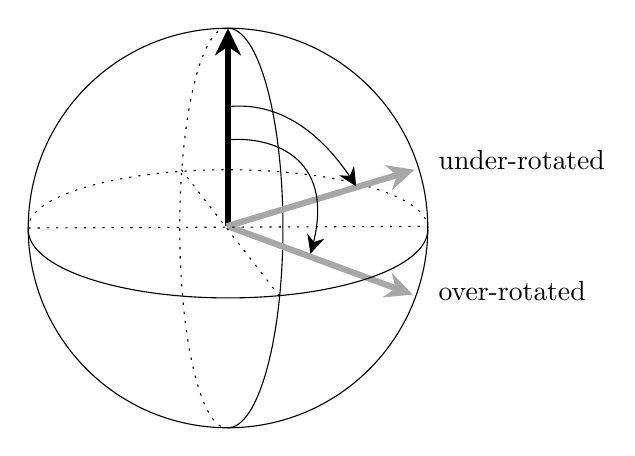
\begin{tikzpicture}[x=0.75pt,y=0.75pt,yscale=-1,xscale=1]
%uncomment if require: \path (0,300); %set diagram left start at 0, and has height of 300

%Shape: Arc [id:dp782370095502481]
\draw  [draw opacity=0][dash pattern={on 0.84pt off 2.51pt}] (212.5,116.75) .. controls (212.5,101.25) and (169.41,88.68) .. (116.25,88.68) .. controls (63.09,88.68) and (20,101.25) .. (20,116.75) .. controls (20,116.75) and (20,116.75) .. (20,116.75) -- (116.25,116.75) -- cycle ; \draw  [dash pattern={on 0.84pt off 2.51pt}] (212.5,116.75) .. controls (212.5,101.25) and (169.41,88.68) .. (116.25,88.68) .. controls (63.09,88.68) and (20,101.25) .. (20,116.75) .. controls (20,116.75) and (20,116.75) .. (20,116.75) ;
%Shape: Circle [id:dp3404154288852026]
\draw   (20,116.75) .. controls (20,63.59) and (63.09,20.5) .. (116.25,20.5) .. controls (169.41,20.5) and (212.5,63.59) .. (212.5,116.75) .. controls (212.5,169.91) and (169.41,213) .. (116.25,213) .. controls (63.09,213) and (20,169.91) .. (20,116.75) -- cycle ;
%Straight Lines [id:da667885384509429]
\draw [line width=2.25]    (116.25,115.95) -- (116.25,25.5) ;
\draw [shift={(116.25,20.5)}, rotate = 450] [fill={rgb, 255:red, 0; green, 0; blue, 0 }  ][line width=0.08]  [draw opacity=0] (13.22,-6.35) -- (0,0) -- (13.22,6.35) -- (8.78,0) -- cycle    ;
%Shape: Arc [id:dp19644604622327155]
\draw  [draw opacity=0] (116.25,20.5) .. controls (116.25,20.5) and (116.25,20.5) .. (116.25,20.5) .. controls (116.25,20.5) and (116.25,20.5) .. (116.25,20.5) .. controls (130.87,20.5) and (142.72,63.59) .. (142.72,116.75) .. controls (142.72,169.91) and (130.87,213) .. (116.25,213) -- (116.25,116.75) -- cycle ; \draw   (116.25,20.5) .. controls (116.25,20.5) and (116.25,20.5) .. (116.25,20.5) .. controls (116.25,20.5) and (116.25,20.5) .. (116.25,20.5) .. controls (130.87,20.5) and (142.72,63.59) .. (142.72,116.75) .. controls (142.72,169.91) and (130.87,213) .. (116.25,213) ;
%Shape: Arc [id:dp34236219446094807]
\draw  [draw opacity=0][dash pattern={on 0.84pt off 2.51pt}] (115.6,20.5) .. controls (115.6,20.5) and (115.6,20.5) .. (115.6,20.5) .. controls (103.13,20.5) and (93.01,63.59) .. (93.01,116.75) .. controls (93.01,169.91) and (103.13,213) .. (115.6,213) -- (115.6,116.75) -- cycle ; \draw  [dash pattern={on 0.84pt off 2.51pt}] (115.6,20.5) .. controls (115.6,20.5) and (115.6,20.5) .. (115.6,20.5) .. controls (103.13,20.5) and (93.01,63.59) .. (93.01,116.75) .. controls (93.01,169.91) and (103.13,213) .. (115.6,213) ;

%Straight Lines [id:da42656322211334885]
\draw [color={rgb, 255:red, 167; green, 167; blue, 167 }  ,draw opacity=1 ][line width=2.25]    (116.25,115.95) -- (200.59,147.1) ;
\draw [shift={(205.28,148.83)}, rotate = 200.27] [fill={rgb, 255:red, 167; green, 167; blue, 167 }  ,fill opacity=1 ][line width=0.08]  [draw opacity=0] (13.22,-6.35) -- (0,0) -- (13.22,6.35) -- (8.78,0) -- cycle    ;
%Straight Lines [id:da7850995960487122]
\draw [color={rgb, 255:red, 167; green, 167; blue, 167 }  ,draw opacity=1 ][line width=2.25]    (115.6,115.95) -- (201.3,90.12) ;
\draw [shift={(206.08,88.68)}, rotate = 523.23] [fill={rgb, 255:red, 167; green, 167; blue, 167 }  ,fill opacity=1 ][line width=0.08]  [draw opacity=0] (13.22,-6.35) -- (0,0) -- (13.22,6.35) -- (8.78,0) -- cycle    ;
%Straight Lines [id:da4695507768944873]
\draw  [dash pattern={on 0.84pt off 2.51pt}]  (93.79,88.68) -- (141.11,149.64) ;
%Straight Lines [id:da7792399094821125]
\draw  [dash pattern={on 0.84pt off 2.51pt}]  (20,116.75) -- (212.5,115.95) ;
%Curve Lines [id:da1883472442634171]
\draw    (117.05,58.2) .. controls (144,55.89) and (163.56,74.28) .. (176.44,94.2) ;
\draw [shift={(178.01,96.7)}, rotate = 238.39] [fill={rgb, 255:red, 0; green, 0; blue, 0 }  ][line width=0.08]  [draw opacity=0] (8.93,-4.29) -- (0,0) -- (8.93,4.29) -- (5.93,0) -- cycle    ;
%Curve Lines [id:da04261734583163235]
\draw    (117.05,74.24) .. controls (134.34,72.67) and (169.36,80.34) .. (156.78,126.32) ;
\draw [shift={(155.95,129.18)}, rotate = 287] [fill={rgb, 255:red, 0; green, 0; blue, 0 }  ][line width=0.08]  [draw opacity=0] (8.93,-4.29) -- (0,0) -- (8.93,4.29) -- (5.93,0) -- cycle    ;
%Shape: Arc [id:dp9372143530929324]
\draw  [draw opacity=0] (212.5,117.55) .. controls (212.5,117.55) and (212.5,117.55) .. (212.5,117.55) .. controls (212.5,117.55) and (212.5,117.55) .. (212.5,117.55) .. controls (212.5,135.71) and (169.41,150.44) .. (116.25,150.44) .. controls (63.09,150.44) and (20,135.71) .. (20,117.55) -- (116.25,117.55) -- cycle ; \draw   (212.5,117.55) .. controls (212.5,117.55) and (212.5,117.55) .. (212.5,117.55) .. controls (212.5,117.55) and (212.5,117.55) .. (212.5,117.55) .. controls (212.5,135.71) and (169.41,150.44) .. (116.25,150.44) .. controls (63.09,150.44) and (20,135.71) .. (20,117.55) ;

% Text Node
\draw (216.48,77.86) node [anchor=north west][inner sep=0.75pt]   [align=left] {under-rotated};
% Text Node
\draw (216.48,141.23) node [anchor=north west][inner sep=0.75pt]   [align=left] {over-rotated};


\end{tikzpicture}

    }
    \hspace{1em}
    \includegraphics[width=.49\textwidth]{phase_transients_viz.png}
    % TODO make this side-by-side and larger
\end{figure}


\end{frame}


\begin{frame}{Magnetic dipolar interactions}

\begin{figure}
\centering
\includegraphics[width=0.4\textwidth]{1H-NMR.jpg}
\hfill
\scalebox{.6}{


\tikzset{every picture/.style={line width=0.75pt}} %set default line width to 0.75pt

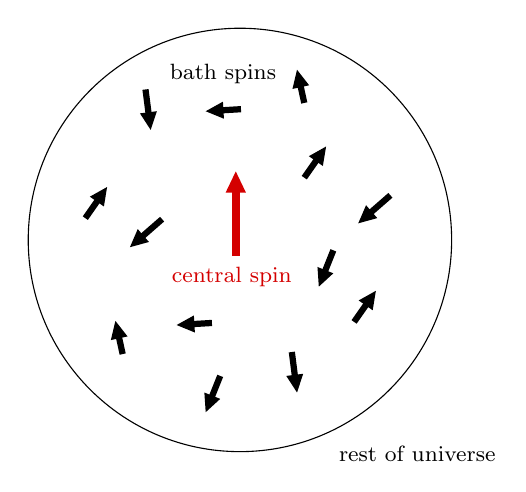
\begin{tikzpicture}[x=0.75pt,y=0.75pt,yscale=-1,xscale=1]
%uncomment if require: \path (0,300); %set diagram left start at 0, and has height of 300

%Shape: Circle [id:dp9038467786645921]
\draw   (10.5,113) .. controls (10.5,56.67) and (56.17,11) .. (112.5,11) .. controls (168.83,11) and (214.5,56.67) .. (214.5,113) .. controls (214.5,169.33) and (168.83,215) .. (112.5,215) .. controls (56.17,215) and (10.5,169.33) .. (10.5,113) -- cycle ;
%Straight Lines [id:da5620058094241265]
\draw [color={rgb, 255:red, 212; green, 0; blue, 0 }  ,draw opacity=1 ][line width=3]    (110.5,120.5) -- (110.5,86) ;
\draw [shift={(110.5,80)}, rotate = 450] [fill={rgb, 255:red, 212; green, 0; blue, 0 }  ,fill opacity=1 ][line width=0.08]  [draw opacity=0] (10.18,-4.89) -- (0,0) -- (10.18,4.89) -- cycle    ;
%Straight Lines [id:da20975151781594947]
\draw [line width=2.25]    (38,102.5) -- (45.63,91.6) ;
\draw [shift={(48.5,87.5)}, rotate = 484.99] [fill={rgb, 255:red, 0; green, 0; blue, 0 }  ][line width=0.08]  [draw opacity=0] (8.57,-4.12) -- (0,0) -- (8.57,4.12) -- cycle    ;
%Straight Lines [id:da3755156093777203]
\draw [line width=2.25]    (167.5,152.5) -- (175.13,141.6) ;
\draw [shift={(178,137.5)}, rotate = 484.99] [fill={rgb, 255:red, 0; green, 0; blue, 0 }  ][line width=0.08]  [draw opacity=0] (8.57,-4.12) -- (0,0) -- (8.57,4.12) -- cycle    ;
%Straight Lines [id:da20398589241562703]
\draw [line width=2.25]    (143.5,83) -- (151.13,72.1) ;
\draw [shift={(154,68)}, rotate = 484.99] [fill={rgb, 255:red, 0; green, 0; blue, 0 }  ][line width=0.08]  [draw opacity=0] (8.57,-4.12) -- (0,0) -- (8.57,4.12) -- cycle    ;
%Straight Lines [id:da2224938850523357]
\draw [line width=2.25]    (143.5,47) -- (141.07,35.88) ;
\draw [shift={(140,31)}, rotate = 437.66] [fill={rgb, 255:red, 0; green, 0; blue, 0 }  ][line width=0.08]  [draw opacity=0] (8.57,-4.12) -- (0,0) -- (8.57,4.12) -- cycle    ;
%Straight Lines [id:da8800601162685735]
\draw [line width=2.25]    (56,168) -- (53.57,156.88) ;
\draw [shift={(52.5,152)}, rotate = 437.66] [fill={rgb, 255:red, 0; green, 0; blue, 0 }  ][line width=0.08]  [draw opacity=0] (8.57,-4.12) -- (0,0) -- (8.57,4.12) -- cycle    ;
%Straight Lines [id:da3276872343023953]
\draw [line width=2.25]    (67,40.5) -- (68.86,55.04) ;
\draw [shift={(69.5,60)}, rotate = 262.69] [fill={rgb, 255:red, 0; green, 0; blue, 0 }  ][line width=0.08]  [draw opacity=0] (8.57,-4.12) -- (0,0) -- (8.57,4.12) -- cycle    ;
%Straight Lines [id:da2341612615458053]
\draw [line width=2.25]    (137.5,167) -- (139.36,181.54) ;
\draw [shift={(140,186.5)}, rotate = 262.69] [fill={rgb, 255:red, 0; green, 0; blue, 0 }  ][line width=0.08]  [draw opacity=0] (8.57,-4.12) -- (0,0) -- (8.57,4.12) -- cycle    ;
%Straight Lines [id:da7637762821470244]
\draw [line width=2.25]    (113,50) -- (100.99,50.71) ;
\draw [shift={(96,51)}, rotate = 356.63] [fill={rgb, 255:red, 0; green, 0; blue, 0 }  ][line width=0.08]  [draw opacity=0] (8.57,-4.12) -- (0,0) -- (8.57,4.12) -- cycle    ;
%Straight Lines [id:da4335342084245668]
\draw [line width=2.25]    (99,153) -- (86.99,153.71) ;
\draw [shift={(82,154)}, rotate = 356.63] [fill={rgb, 255:red, 0; green, 0; blue, 0 }  ][line width=0.08]  [draw opacity=0] (8.57,-4.12) -- (0,0) -- (8.57,4.12) -- cycle    ;
%Straight Lines [id:da6429700423794917]
\draw [line width=2.25]    (185,91.5) -- (173.27,101.72) ;
\draw [shift={(169.5,105)}, rotate = 318.95] [fill={rgb, 255:red, 0; green, 0; blue, 0 }  ][line width=0.08]  [draw opacity=0] (8.57,-4.12) -- (0,0) -- (8.57,4.12) -- cycle    ;
%Straight Lines [id:da08886387795812767]
\draw [line width=2.25]    (75,103) -- (63.27,113.22) ;
\draw [shift={(59.5,116.5)}, rotate = 318.95] [fill={rgb, 255:red, 0; green, 0; blue, 0 }  ][line width=0.08]  [draw opacity=0] (8.57,-4.12) -- (0,0) -- (8.57,4.12) -- cycle    ;
%Straight Lines [id:da711271255542824]
\draw [line width=2.25]    (103,178.5) -- (97.86,191.36) ;
\draw [shift={(96,196)}, rotate = 291.8] [fill={rgb, 255:red, 0; green, 0; blue, 0 }  ][line width=0.08]  [draw opacity=0] (8.57,-4.12) -- (0,0) -- (8.57,4.12) -- cycle    ;
%Straight Lines [id:da5759228221019161]
\draw [line width=2.25]    (157.5,118) -- (152.36,130.86) ;
\draw [shift={(150.5,135.5)}, rotate = 291.8] [fill={rgb, 255:red, 0; green, 0; blue, 0 }  ][line width=0.08]  [draw opacity=0] (8.57,-4.12) -- (0,0) -- (8.57,4.12) -- cycle    ;

% Text Node
\draw (78.5,125) node [anchor=north west][inner sep=0.75pt]  [font=\footnotesize,color={rgb, 255:red, 212; green, 0; blue, 0 }  ,opacity=1 ] [align=left] {central spin};
% Text Node
\draw (77.5,27) node [anchor=north west][inner sep=0.75pt]  [font=\footnotesize] [align=left] {bath spins};
% Text Node
\draw (159,211) node [anchor=north west][inner sep=0.75pt]  [font=\footnotesize] [align=left] {rest of universe};


\end{tikzpicture}

}
\end{figure}
\vspace{-1em}
\hspace{3em}
{\scriptsize%
% for NMR spectrum figure
\nocite{Ottowa-NMR}
From Facey 2008.%
}

Magentic dipolar interactions $H_D$\dots
\begin{itemize}
    \item Broaden spectral lines in NMR
    \item Lead to decay of central spin coherence in bath
\end{itemize}

Don't want dipolar interactions! Decoupling (removing) them would narrow spectral lines and increase coherence times.


\end{frame}

\section{Hamiltonian engineering}


\begin{frame}{Hamiltonian engineering}

% set up Hamiltonian engineering

\[
H(t) = H_{\text{sys}} + H_{\text{ctrl}}(t)
\]

Goal: ``engineer'' an effective Hamiltonian $H_{\text{eff}}$ using $H_{\text{ctrl}}(t)$

\[
U(T) = Te^{-i \int_0^T H(t) dt } = e^{-i H_{\text{eff}} T}
\]

% TODO Bloch sphere example showing ideal6 or something for time suspension
\begin{figure}
$H_{\text{eff}} = 0$ \\
\includegraphics[width=.5\textwidth]{hamiltonian_engineering.jpeg}
\end{figure}


\note{
Hamiltonian engineering used for:

\begin{itemize}
    \item Sensing (decoupling dipolar interactions while keeping chemical shift, e.g. $H_\text{eff} = \beta \textcolor[rgb]{0,0.69,0}{H_{\text{CS}}}$)
    \item Quantum memory (decoupling all interactions, $H_\text{eff} = 0$)
    \item Quantum simulation
\end{itemize}
}

\end{frame}




\begin{frame}{Average Hamiltonian theory (AHT)}

The time-evolution operator (or propagator) characterizes time-evolution of states
\[
\ket{\psi(t)} = U(t)\ket{\psi(0)}, \rho(t) = U(t) \rho(0) U^\dagger(t)
\]
and follows the differential equation
\[
i \frac{d}{dt} U(t) = H(t)U(t)
\]
\[
U(0) = \identity
\]

The Magnus Expansion gives an exponential solution for $U(t)$
via an \emph{average Hamiltonian} $\overline{H}$ at time $t$ \cite{Blanes_2009,2010EJPh...31..907B}
\[
U(t) = e^{-i \overline{H} t}
\]
with $\overline{H} = \overline{H}^{(0)} + \overline{H}^{(1)} + \dots$.

\[
\overline{H}^{(0)} = \frac{1}{T} \int_0^{T}
    H(t) dt
\]

The series converges rapidly when $t||H|| \ll 1$.
% TODO check ^, replace with more formal statement from thesis

\end{frame}

\begin{frame}{AHT: interaction frame}

What if $t||H||$ is large (strong pulses from $H_{\text{ctrl}}$)? Go into the interaction frame! \cite{brinkmann_2016}

\begin{align*}
    \frac{d}{dt} U_{\text{ctrl}}(t) &=
        -i H_{\text{ctrl}}(t)U_{\text{ctrl}}(t) \\
    U_{\text{ctrl}}(0) &= \identity
\end{align*}

So the Hamiltonian in the interaction frame becomes

\[
    \widetilde{H}(t) = \widetilde{H}_{\text{sys}}(t) = U_{\text{ctrl}}(t)^\dagger H_{\text{sys}} U_{\text{ctrl}}(t)
\]

\end{frame}

\begin{frame}{AHT: Pulse sequences}

If a pulse sequence is both cyclic and periodic \cite{gerstein-dybowski}
\begin{align*}
    U_{\text{ctrl}}(T) &= T\exp \left(
        -i \int_0^{T} H_{\text{ctrl}}(t) dt \right) = \pm \identity
         \, \text{(cyclic)} \\
    H_{\text{ctrl}}(t) &= H_{\text{ctrl}}(t + NT) \, \text{(periodic)}
\end{align*}
then the interaction frame and the lab frame coincide at multiples of
the cycle time, and the propagator can be given by
\[
    U(T) = \exp\left( -i T (\overline{H}^{(0)} +
        \overline{H}^{(1)} + \dots) \right)
\]
% Higher-order terms for average Hamiltonian become nasty\dots

\end{frame}


\begin{frame}{Average Hamiltonian theory (AHT)}

% If\dots
% \begin{itemize}
%     \item Consider cyclic and periodic pulse sequences
%     \[
%     U_{\text{ctrl}}(T) = \identity, H_{\text{ctrl}}(t) = H_{\text{ctrl}}(t + NT)
%     \]
%     \item Observe system stroboscopically ($t = NT$)
% \end{itemize}
% \dots then system appears to evolve under an effective \emph{average} Hamiltonian.
% TODO does this make sense in context of above?

\begin{figure}
\centering
\scalebox{.7}{
\tikzset{every picture/.style={line width=0.75pt}} %set default line width to 0.75pt

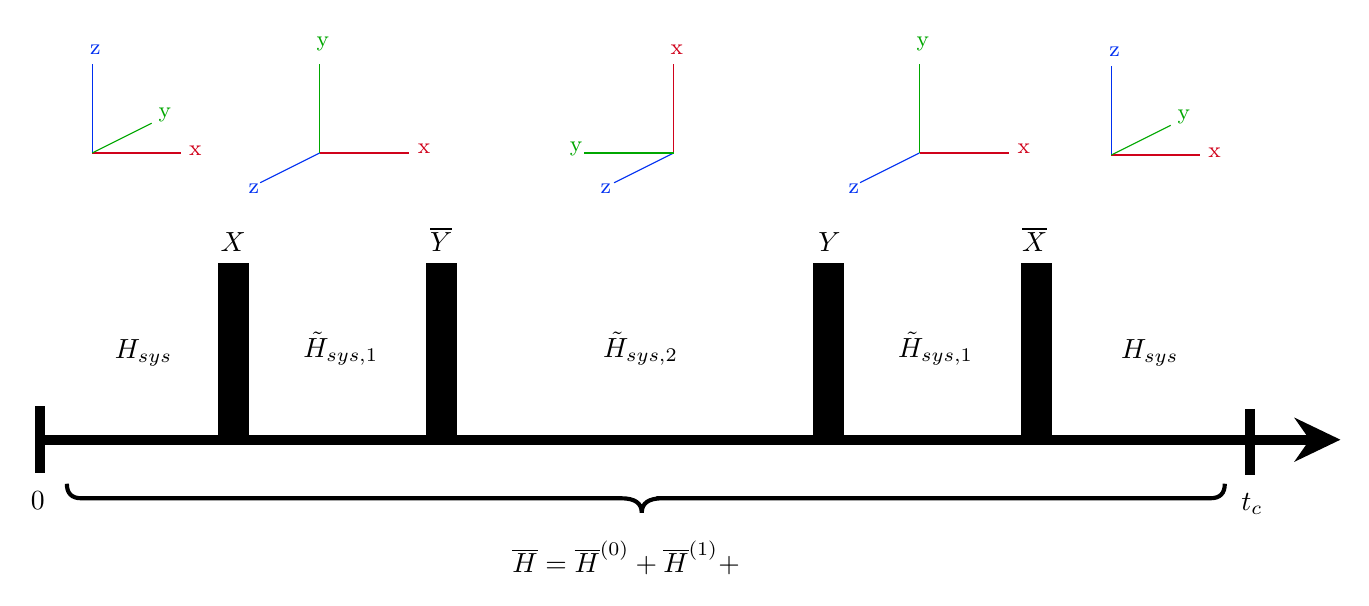
\begin{tikzpicture}[x=0.75pt,y=0.75pt,yscale=-1,xscale=1]
%uncomment if require: \path (0,327); %set diagram left start at 0, and has height of 327

%Shape: Rectangle [id:dp757529732417089]
\draw  [fill={rgb, 255:red, 0; green, 0; blue, 0 }  ,fill opacity=1 ] (101.1,123.91) -- (115.43,123.91) -- (115.43,209.89) -- (101.1,209.89) -- cycle ;
%Straight Lines [id:da8398663533091074]
\draw [line width=3.75]    (15.12,208.75) -- (634.62,208.75) ;
\draw [shift={(641.62,208.75)}, rotate = 180] [fill={rgb, 255:red, 0; green, 0; blue, 0 }  ][line width=0.08]  [draw opacity=0] (22.33,-10.72) -- (0,0) -- (22.33,10.73) -- (14.83,0) -- cycle    ;
%Shape: Rectangle [id:dp8989097393091372]
\draw  [fill={rgb, 255:red, 0; green, 0; blue, 0 }  ,fill opacity=1 ] (201.41,123.91) -- (215.74,123.91) -- (215.74,209.89) -- (201.41,209.89) -- cycle ;
%Shape: Rectangle [id:dp5203891268410358]
\draw  [fill={rgb, 255:red, 0; green, 0; blue, 0 }  ,fill opacity=1 ] (387.69,123.91) -- (402.02,123.91) -- (402.02,209.89) -- (387.69,209.89) -- cycle ;
%Shape: Rectangle [id:dp5922766644502158]
\draw  [fill={rgb, 255:red, 0; green, 0; blue, 0 }  ,fill opacity=1 ] (488,123.91) -- (502.33,123.91) -- (502.33,209.89) -- (488,209.89) -- cycle ;
%Shape: Brace [id:dp004729490444473794]
\draw  [line width=1.5]  (28.02,229.96) .. controls (28.02,234.63) and (30.35,236.96) .. (35.02,236.96) -- (295,236.96) .. controls (301.67,236.96) and (305,239.29) .. (305,243.96) .. controls (305,239.29) and (308.33,236.96) .. (315,236.96)(312,236.96) -- (578.92,236.96) .. controls (583.59,236.96) and (585.92,234.63) .. (585.92,229.96) ;
%Straight Lines [id:da5692356671850871]
\draw [color={rgb, 255:red, 208; green, 2; blue, 27 }  ,draw opacity=1 ]   (40.21,70.6) -- (83.2,70.6) ;
%Straight Lines [id:da6810769300954256]
\draw [color={rgb, 255:red, 0; green, 47; blue, 241 }  ,draw opacity=1 ]   (40.21,70.6) -- (40.21,27.61) ;
%Straight Lines [id:da050165915493954216]
\draw [color={rgb, 255:red, 0; green, 167; blue, 0 }  ,draw opacity=1 ]   (40.21,70.6) -- (68.87,56.27) ;

%Straight Lines [id:da5081204556289702]
\draw [color={rgb, 255:red, 208; green, 2; blue, 27 }  ,draw opacity=1 ]   (149.82,70.6) -- (192.81,70.6) ;
%Straight Lines [id:da6854547629628449]
\draw [color={rgb, 255:red, 0; green, 47; blue, 241 }  ,draw opacity=1 ]   (149.82,70.6) -- (121.16,84.93) ;
%Straight Lines [id:da7186146502407351]
\draw [color={rgb, 255:red, 0; green, 167; blue, 0 }  ,draw opacity=1 ]   (149.82,70.6) -- (149.82,27.61) ;

%Straight Lines [id:da24563094299910881]
\draw [color={rgb, 255:red, 208; green, 2; blue, 27 }  ,draw opacity=1 ]   (320.34,70.6) -- (320.34,27.61) ;
%Straight Lines [id:da179977702531384]
\draw [color={rgb, 255:red, 0; green, 47; blue, 241 }  ,draw opacity=1 ]   (320.34,70.6) -- (291.68,84.93) ;
%Straight Lines [id:da7516580599441232]
\draw [color={rgb, 255:red, 0; green, 167; blue, 0 }  ,draw opacity=1 ]   (320.34,70.6) -- (277.35,70.6) ;

%Straight Lines [id:da5137007458732086]
\draw [line width=3.75]    (598.05,193.84) -- (598.05,225.94) ;
%Straight Lines [id:da9300296101367684]
\draw [line width=3.75]    (15.12,192.7) -- (15.12,224.8) ;
%Straight Lines [id:da0881233734207878]
\draw [color={rgb, 255:red, 208; green, 2; blue, 27 }  ,draw opacity=1 ]   (531.21,71.6) -- (574.2,71.6) ;
%Straight Lines [id:da9374652913281989]
\draw [color={rgb, 255:red, 0; green, 47; blue, 241 }  ,draw opacity=1 ]   (531.21,71.6) -- (531.21,28.61) ;
%Straight Lines [id:da610003280154453]
\draw [color={rgb, 255:red, 0; green, 167; blue, 0 }  ,draw opacity=1 ]   (531.21,71.6) -- (559.87,57.27) ;

%Straight Lines [id:da5081271261395761]
\draw [color={rgb, 255:red, 208; green, 2; blue, 27 }  ,draw opacity=1 ]   (438.82,70.6) -- (481.81,70.6) ;
%Straight Lines [id:da9429921450367487]
\draw [color={rgb, 255:red, 0; green, 47; blue, 241 }  ,draw opacity=1 ]   (438.82,70.6) -- (410.16,84.93) ;
%Straight Lines [id:da28825440756966425]
\draw [color={rgb, 255:red, 0; green, 167; blue, 0 }  ,draw opacity=1 ]   (438.82,70.6) -- (438.82,27.61) ;


% Text Node
\draw (108.11,113.73) node  [font=\normalsize] [align=left] {$\displaystyle X$};
% Text Node
\draw (208.42,112.3) node  [font=\normalsize] [align=left] {$\displaystyle \overline{Y}$};
% Text Node
\draw (494.3,112.3) node  [font=\normalsize] [align=left] {$\displaystyle \overline{X}$};
% Text Node
\draw (395.43,113.73) node  [font=\normalsize] [align=left] {$\displaystyle Y$};
% Text Node
\draw (592.63,233.46) node [anchor=north west][inner sep=0.75pt]  [font=\normalsize]  {$t_{c}$};
% Text Node
\draw (9.41,232.39) node [anchor=north west][inner sep=0.75pt]  [font=\normalsize]  {$0$};
% Text Node
\draw (64.99,166.9) node  [font=\normalsize]  {$H_{\text{sys}}$};
% Text Node
\draw (160,164.75) node  [font=\normalsize]  {$\tilde{H}_{\text{sys, 1}}$};
% Text Node
\draw (304.44,164.75) node  [font=\normalsize]  {$\tilde{H}_{\text{sys, 2}}$};
% Text Node
\draw (446.59,164.75) node  [font=\normalsize]  {$\tilde{H}_{\text{sys, 1}}$};
% Text Node
\draw (549.77,166.9) node  [font=\normalsize]  {$H_{\text{sys}}$};
% Text Node
\draw (241.4,256.21) node [anchor=north west][inner sep=0.75pt]  [font=\normalsize]  {$\overline{H} =\overline{H}^{( 0)} +\overline{H}^{( 1)} +\dotsc $};
% Text Node
\draw (89.95,69.6) node  [font=\footnotesize,color={rgb, 255:red, 208; green, 2; blue, 27 }  ,opacity=1 ] [align=left] {x};
% Text Node
\draw (75.19,52.4) node  [font=\footnotesize,color={rgb, 255:red, 0; green, 167; blue, 0 }  ,opacity=1 ] [align=left] {y};
% Text Node
\draw (41.79,20.87) node  [font=\footnotesize,color={rgb, 255:red, 0; green, 47; blue, 241 }  ,opacity=1 ] [align=left] {z};
% Text Node
\draw (200.12,68.6) node  [font=\footnotesize,color={rgb, 255:red, 208; green, 2; blue, 27 }  ,opacity=1 ] [align=left] {x};
% Text Node
\draw (151.4,18.01) node  [font=\footnotesize,color={rgb, 255:red, 0; green, 167; blue, 0 }  ,opacity=1 ] [align=left] {y};
% Text Node
\draw (118.16,87.93) node  [font=\footnotesize,color={rgb, 255:red, 0; green, 47; blue, 241 }  ,opacity=1 ] [align=left] {z};
% Text Node
\draw (321.93,20.87) node  [font=\footnotesize,color={rgb, 255:red, 208; green, 2; blue, 27 }  ,opacity=1 ] [align=left] {x};
% Text Node
\draw (273.35,68.6) node  [font=\footnotesize,color={rgb, 255:red, 0; green, 167; blue, 0 }  ,opacity=1 ] [align=left] {y};
% Text Node
\draw (287.68,87.93) node  [font=\footnotesize,color={rgb, 255:red, 0; green, 47; blue, 241 }  ,opacity=1 ] [align=left] {z};
% Text Node
\draw (407.16,87.93) node  [font=\footnotesize,color={rgb, 255:red, 0; green, 47; blue, 241 }  ,opacity=1 ] [align=left] {z};
% Text Node
\draw (440.4,18.01) node  [font=\footnotesize,color={rgb, 255:red, 0; green, 167; blue, 0 }  ,opacity=1 ] [align=left] {y};
% Text Node
\draw (489.12,68.6) node  [font=\footnotesize,color={rgb, 255:red, 208; green, 2; blue, 27 }  ,opacity=1 ] [align=left] {x};
% Text Node
\draw (532.79,21.87) node  [font=\footnotesize,color={rgb, 255:red, 0; green, 47; blue, 241 }  ,opacity=1 ] [align=left] {z};
% Text Node
\draw (566.19,53.4) node  [font=\footnotesize,color={rgb, 255:red, 0; green, 167; blue, 0 }  ,opacity=1 ] [align=left] {y};
% Text Node
\draw (580.95,70.6) node  [font=\footnotesize,color={rgb, 255:red, 208; green, 2; blue, 27 }  ,opacity=1 ] [align=left] {x};


\end{tikzpicture}

}
\end{figure}
% and include diagram showing difficulty with different time terms

\note{
Average Hamiltonian Theory (AHT) has been used extensively for Hamiltonian engineering. AHT lets you design pulse sequences that decouples (cancels) certain terms in the Hamiltonian.

Axes in the figure show the orientation of the interaction frame, cyclic because first and last orientations are the same.

If you measure at $T$, then system will appear to evolve under $\overline{H}$.

% Interaction frame is determined by $H_{\text{ctrl}}$, ``toggles'' the system Hamiltonian.

% Note how the first-order term has commutator of toggled Hamiltonians at different times. This is straightforward to calculate with a 4-pulse sequence, but gets analytically intractable for longer sequences, and for higher-order terms.
}

\end{frame}

\begin{frame}{Existing AHT approaches to Hamiltonian engineering}

\begin{itemize}
    \item WAHUHA 4-pulse sequence (\cite{PhysRevLett.20.180}), decouples dipolar interaction to lowest-order

    \item CORY 48-pulse sequence (\cite{CORY1990205}) designed analytically using AHT to be robust to experimental imperfections, decouples \emph{all} interactions to second order
\end{itemize}

\begin{figure}
\centering
\includegraphics[width=.7\textwidth]{decay_plot.pdf}
\end{figure}

\note{
WHH-4 designed with pen and paper

Plot of average correlation of adamantane sample for FID, and using two pulse sequences. See how coherence time improves with dipolar decoupling! But there's still room to improve before we reach T1 limit.

}

\end{frame}

\begin{frame}{AHT limitations}

{\scriptsize % or \footnotesize
\begin{align*}
    \overline{H}^{(0)} &= \frac{1}{T} \int_0^{T}
        \widetilde{H}_{\text{sys}}(t) dt \\
    %
    \overline{H}^{(1)} &= \frac{1}{2iT} \int_0^{T} dt_1 \int_0^{t_1} dt_2
        \left[\widetilde{H}_{\text{sys}}(t_1), \widetilde{H}_{\text{sys}}(t_2)\right] \\
    %
    \overline{H}^{(2)} &= -\frac{1}{6T}
    \int_0^{T} dt_1 \int_0^{t_1} dt_2 \int_0^{t_2} dt_3
    \left\{
    \left[\widetilde{H}_{\text{sys}}(t_1), \left[\widetilde{H}_{\text{sys}}(t_2), \widetilde{H}_{\text{sys}}(t_3)\right]\right] \right. \\
    & \hspace{13em} + \left.
    \left[\left[\widetilde{H}_{\text{sys}}(t_1), \widetilde{H}_{\text{sys}}(t_2)\right], \widetilde{H}_{\text{sys}}(t_3)\right]
    \right\}
\end{align*}
}
\vspace{-1em}
\begin{figure}
\centering
\includegraphics[width=0.3\textwidth]{AHT-HO-diagram.pdf}

{\scriptsize From \cite{brinkmann_2016}.}
\end{figure}
% TODO make sure I can see this figure ^

\note{

AHT is great, but it gets really hard to calculate higher order terms (especially for longer pulse sequences).

``RL has been advancing rapidly in recent years, useful tool for tackling a wide range of problems''

Are there better approaches to Hamiltonian engineering using RL?
}

\end{frame}


\begin{frame}{AHT limitations}


\emph{Is there a better way?}

\end{frame}



\section{Reinforcement learning (RL) for Hamiltonian engineering}

\begin{frame}{Reinforcement learning}

\begin{figure}
\centering
\includegraphics[width=.8\textwidth]{rl.png}

From \cite{sutton2018reinforcement}.
\end{figure}

\begin{figure}
\centering
\includegraphics[width=.4\textwidth]{tetris.png}
\end{figure}

\end{frame}


\begin{frame}{RL for Hamiltonian engineering}
%










% TODO continue...





\begin{itemize}
    \item State $\to$ sequence of pulses
    \item Action $\to$ control pulse ($\{ D, X, \overline{X}, Y, \overline{Y} \}$)
    \item Reward $\to$ propagator fidelity
\end{itemize}

\[
\text{fidelity} = \left(\Re{
    \frac{\Tr{U_\text{target}^\dagger U(t)}}{\Tr{\identity}}
}\right)
\]
% TODO double check if I'm using this or average gate fidelity

Actually use log transformation of fidelity
\[
r = -\log(1 - \text{fidelity})
\]

% TODO add visual

\note{
With RL, potential for tailored pulse sequences for particular systems (e.g. strongly coupled vs weakly coupled), learned robustness to errors.
}


\end{frame}


\begin{frame}{AlphaZero Algorithm}

Tried \emph{many} different RL algorithms for pulse sequence design, AlphaZero algorithm (\cite{Silver1140}, originally for Chess, Shogi, and Go) performed the best.

\begin{figure}
\centering
\includegraphics[width=.8\textwidth]{az-parallel.jpeg}
% TODO update this diagram
\end{figure}

\note{

% Each iteration of algorithm involves collecting data in a tree search and training neural networks on the collected data. Neural network maps state to policy (what pulse should I apply next?) and value (how good will this pulse sequence be?).

With tree structure, can optionally add AHT constraints to search.

% Collects data on pulse sequences, balancing \emph{exploration} of new
% pulse sequences and \emph{exploitation} of learnings (via neural
% networks), and trains neural networks on collected data to learn from
% recent experiences.
}

\end{frame}



\begin{frame}[allowframebreaks]{AlphaZero: tree search}

% \begin{figure}
% \centering
% \scalebox{.7}{
% 

\tikzset{every picture/.style={line width=0.75pt}} %set default line width to 0.75pt

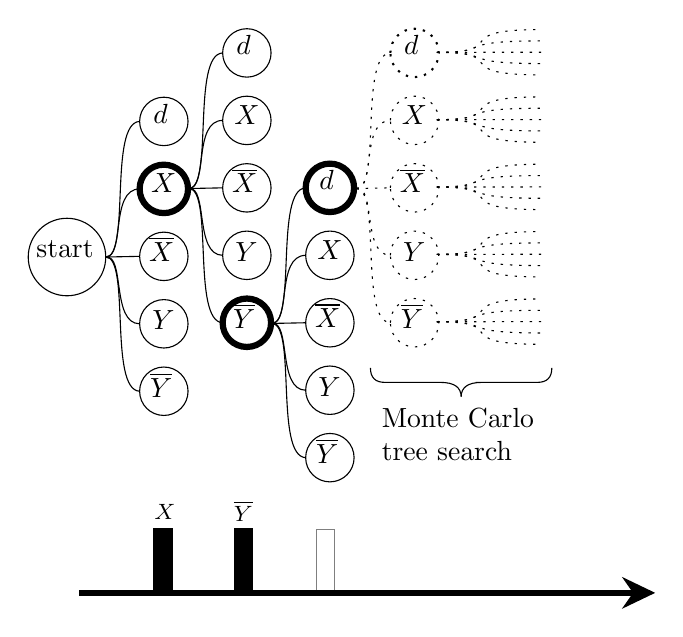
\begin{tikzpicture}[x=0.75pt,y=0.75pt,yscale=-1,xscale=1]
%uncomment if require: \path (0,300); %set diagram left start at 0, and has height of 300

%Shape: Circle [id:dp9046759261625568]
\draw   (77,60.67) .. controls (77,54.22) and (82.22,49) .. (88.67,49) .. controls (95.11,49) and (100.33,54.22) .. (100.33,60.67) .. controls (100.33,67.11) and (95.11,72.33) .. (88.67,72.33) .. controls (82.22,72.33) and (77,67.11) .. (77,60.67) -- cycle ;
%Shape: Circle [id:dp2720164009687023]
\draw  [line width=2.25]  (77,93.17) .. controls (77,86.73) and (82.22,81.5) .. (88.67,81.5) .. controls (95.11,81.5) and (100.33,86.73) .. (100.33,93.17) .. controls (100.33,99.61) and (95.11,104.84) .. (88.67,104.84) .. controls (82.22,104.84) and (77,99.61) .. (77,93.17) -- cycle ;
%Shape: Circle [id:dp7036273582393138]
\draw   (77,125.67) .. controls (77,119.23) and (82.22,114.01) .. (88.67,114.01) .. controls (95.11,114.01) and (100.33,119.23) .. (100.33,125.67) .. controls (100.33,132.12) and (95.11,137.34) .. (88.67,137.34) .. controls (82.22,137.34) and (77,132.12) .. (77,125.67) -- cycle ;
%Shape: Circle [id:dp30398985571820214]
\draw   (77,158.18) .. controls (77,151.73) and (82.22,146.51) .. (88.67,146.51) .. controls (95.11,146.51) and (100.33,151.73) .. (100.33,158.18) .. controls (100.33,164.62) and (95.11,169.84) .. (88.67,169.84) .. controls (82.22,169.84) and (77,164.62) .. (77,158.18) -- cycle ;
%Shape: Circle [id:dp47733742173317295]
\draw   (77,190.67) .. controls (77,184.22) and (82.22,179) .. (88.67,179) .. controls (95.11,179) and (100.33,184.22) .. (100.33,190.67) .. controls (100.33,197.11) and (95.11,202.33) .. (88.67,202.33) .. controls (82.22,202.33) and (77,197.11) .. (77,190.67) -- cycle ;
%Curve Lines [id:da15003157478518636]
\draw    (60.67,126) .. controls (72.67,126) and (62,61.33) .. (77,60.67) ;
%Curve Lines [id:da8250791502123043]
\draw    (60.67,126) .. controls (70,126) and (62.67,93.33) .. (77,93.17) ;
%Curve Lines [id:da9035503948679597]
\draw    (60.67,126) .. controls (72.67,126) and (62,189.97) .. (77,190.67) ;
%Curve Lines [id:da20495653155266225]
\draw    (60.67,126) .. controls (70,124.67) and (63.33,158) .. (77,158.18) ;
%Straight Lines [id:da5161405015219109]
\draw    (60.67,126) -- (77,125.67) ;

%Shape: Circle [id:dp6856566096163164]
\draw   (23.33,126) .. controls (23.33,115.69) and (31.69,107.33) .. (42,107.33) .. controls (52.31,107.33) and (60.67,115.69) .. (60.67,126) .. controls (60.67,136.31) and (52.31,144.67) .. (42,144.67) .. controls (31.69,144.67) and (23.33,136.31) .. (23.33,126) -- cycle ;
%Shape: Circle [id:dp3943399377951582]
\draw   (117,27.67) .. controls (117,21.22) and (122.22,16) .. (128.67,16) .. controls (135.11,16) and (140.33,21.22) .. (140.33,27.67) .. controls (140.33,34.11) and (135.11,39.33) .. (128.67,39.33) .. controls (122.22,39.33) and (117,34.11) .. (117,27.67) -- cycle ;
%Shape: Circle [id:dp027403378825546554]
\draw   (117,60.17) .. controls (117,53.73) and (122.22,48.5) .. (128.67,48.5) .. controls (135.11,48.5) and (140.33,53.73) .. (140.33,60.17) .. controls (140.33,66.61) and (135.11,71.84) .. (128.67,71.84) .. controls (122.22,71.84) and (117,66.61) .. (117,60.17) -- cycle ;
%Shape: Circle [id:dp18742338383587276]
\draw   (117,92.67) .. controls (117,86.23) and (122.22,81.01) .. (128.67,81.01) .. controls (135.11,81.01) and (140.33,86.23) .. (140.33,92.67) .. controls (140.33,99.12) and (135.11,104.34) .. (128.67,104.34) .. controls (122.22,104.34) and (117,99.12) .. (117,92.67) -- cycle ;
%Shape: Circle [id:dp9772441176859072]
\draw   (117,125.18) .. controls (117,118.73) and (122.22,113.51) .. (128.67,113.51) .. controls (135.11,113.51) and (140.33,118.73) .. (140.33,125.18) .. controls (140.33,131.62) and (135.11,136.84) .. (128.67,136.84) .. controls (122.22,136.84) and (117,131.62) .. (117,125.18) -- cycle ;
%Shape: Circle [id:dp6375454025693941]
\draw  [line width=2.25]  (117,157.67) .. controls (117,151.22) and (122.22,146) .. (128.67,146) .. controls (135.11,146) and (140.33,151.22) .. (140.33,157.67) .. controls (140.33,164.11) and (135.11,169.33) .. (128.67,169.33) .. controls (122.22,169.33) and (117,164.11) .. (117,157.67) -- cycle ;
%Curve Lines [id:da7935513938946654]
\draw    (100.67,93) .. controls (112.67,93) and (102,28.33) .. (117,27.67) ;
%Curve Lines [id:da9090746048189753]
\draw    (100.67,93) .. controls (110,93) and (102.67,60.33) .. (117,60.17) ;
%Curve Lines [id:da08019414129507907]
\draw    (100.67,93) .. controls (112.67,93) and (102,156.97) .. (117,157.67) ;
%Curve Lines [id:da8818934103423806]
\draw    (100.67,93) .. controls (110,91.67) and (103.33,125) .. (117,125.18) ;
%Straight Lines [id:da3600527836975942]
\draw    (100.67,93) -- (117,92.67) ;

%Shape: Circle [id:dp37197107969313614]
\draw  [line width=2.25]  (157,92.67) .. controls (157,86.22) and (162.22,81) .. (168.67,81) .. controls (175.11,81) and (180.33,86.22) .. (180.33,92.67) .. controls (180.33,99.11) and (175.11,104.33) .. (168.67,104.33) .. controls (162.22,104.33) and (157,99.11) .. (157,92.67) -- cycle ;
%Shape: Circle [id:dp6275475319115866]
\draw   (157,125.17) .. controls (157,118.73) and (162.22,113.5) .. (168.67,113.5) .. controls (175.11,113.5) and (180.33,118.73) .. (180.33,125.17) .. controls (180.33,131.61) and (175.11,136.84) .. (168.67,136.84) .. controls (162.22,136.84) and (157,131.61) .. (157,125.17) -- cycle ;
%Shape: Circle [id:dp20634171892967257]
\draw   (157,157.67) .. controls (157,151.23) and (162.22,146.01) .. (168.67,146.01) .. controls (175.11,146.01) and (180.33,151.23) .. (180.33,157.67) .. controls (180.33,164.12) and (175.11,169.34) .. (168.67,169.34) .. controls (162.22,169.34) and (157,164.12) .. (157,157.67) -- cycle ;
%Shape: Circle [id:dp005375931541727663]
\draw   (157,190.18) .. controls (157,183.73) and (162.22,178.51) .. (168.67,178.51) .. controls (175.11,178.51) and (180.33,183.73) .. (180.33,190.18) .. controls (180.33,196.62) and (175.11,201.84) .. (168.67,201.84) .. controls (162.22,201.84) and (157,196.62) .. (157,190.18) -- cycle ;
%Shape: Circle [id:dp30698472035152635]
\draw   (157,222.67) .. controls (157,216.22) and (162.22,211) .. (168.67,211) .. controls (175.11,211) and (180.33,216.22) .. (180.33,222.67) .. controls (180.33,229.11) and (175.11,234.33) .. (168.67,234.33) .. controls (162.22,234.33) and (157,229.11) .. (157,222.67) -- cycle ;
%Curve Lines [id:da24565594693868897]
\draw    (140.67,158) .. controls (152.67,158) and (142,93.33) .. (157,92.67) ;
%Curve Lines [id:da5338540044019582]
\draw    (140.67,158) .. controls (150,158) and (142.67,125.33) .. (157,125.17) ;
%Curve Lines [id:da9225241366716022]
\draw    (140.67,158) .. controls (152.67,158) and (142,221.97) .. (157,222.67) ;
%Curve Lines [id:da15552356993518202]
\draw    (140.67,158) .. controls (150,156.67) and (143.33,190) .. (157,190.18) ;
%Straight Lines [id:da21353471154132975]
\draw    (140.67,158) -- (157,157.67) ;

%Shape: Circle [id:dp04181875688613368]
\draw  [dash pattern={on 0.84pt off 2.51pt}][line width=0.75]  (197.8,27.67) .. controls (197.8,21.22) and (203.02,16) .. (209.47,16) .. controls (215.91,16) and (221.13,21.22) .. (221.13,27.67) .. controls (221.13,34.11) and (215.91,39.33) .. (209.47,39.33) .. controls (203.02,39.33) and (197.8,34.11) .. (197.8,27.67) -- cycle ;
%Shape: Circle [id:dp9520151357098714]
\draw  [dash pattern={on 0.84pt off 2.51pt}] (197.8,60.17) .. controls (197.8,53.73) and (203.02,48.5) .. (209.47,48.5) .. controls (215.91,48.5) and (221.13,53.73) .. (221.13,60.17) .. controls (221.13,66.61) and (215.91,71.84) .. (209.47,71.84) .. controls (203.02,71.84) and (197.8,66.61) .. (197.8,60.17) -- cycle ;
%Shape: Circle [id:dp6091644032597949]
\draw  [dash pattern={on 0.84pt off 2.51pt}] (197.8,92.67) .. controls (197.8,86.23) and (203.02,81.01) .. (209.47,81.01) .. controls (215.91,81.01) and (221.13,86.23) .. (221.13,92.67) .. controls (221.13,99.12) and (215.91,104.34) .. (209.47,104.34) .. controls (203.02,104.34) and (197.8,99.12) .. (197.8,92.67) -- cycle ;
%Shape: Circle [id:dp30106591129563065]
\draw  [dash pattern={on 0.84pt off 2.51pt}] (197.8,125.18) .. controls (197.8,118.73) and (203.02,113.51) .. (209.47,113.51) .. controls (215.91,113.51) and (221.13,118.73) .. (221.13,125.18) .. controls (221.13,131.62) and (215.91,136.84) .. (209.47,136.84) .. controls (203.02,136.84) and (197.8,131.62) .. (197.8,125.18) -- cycle ;
%Shape: Circle [id:dp11491575042636026]
\draw  [dash pattern={on 0.84pt off 2.51pt}] (197.8,157.67) .. controls (197.8,151.22) and (203.02,146) .. (209.47,146) .. controls (215.91,146) and (221.13,151.22) .. (221.13,157.67) .. controls (221.13,164.11) and (215.91,169.33) .. (209.47,169.33) .. controls (203.02,169.33) and (197.8,164.11) .. (197.8,157.67) -- cycle ;
%Curve Lines [id:da6833103888584182]
\draw  [dash pattern={on 0.84pt off 2.51pt}]  (181.47,93) .. controls (193.47,93) and (182.8,28.33) .. (197.8,27.67) ;
%Curve Lines [id:da7170577068303761]
\draw  [dash pattern={on 0.84pt off 2.51pt}]  (181.47,93) .. controls (190.8,93) and (183.47,60.33) .. (197.8,60.17) ;
%Curve Lines [id:da9592178971273932]
\draw  [dash pattern={on 0.84pt off 2.51pt}]  (181.47,93) .. controls (193.47,93) and (182.8,156.97) .. (197.8,157.67) ;
%Curve Lines [id:da8897306480704943]
\draw  [dash pattern={on 0.84pt off 2.51pt}]  (181.47,93) .. controls (190.8,91.67) and (184.13,125) .. (197.8,125.18) ;
%Straight Lines [id:da5951582855021698]
\draw  [dash pattern={on 0.84pt off 2.51pt}]  (181.47,93) -- (197.8,92.67) ;
%Curve Lines [id:da8597674854104052]
\draw  [dash pattern={on 0.84pt off 2.51pt}]  (220.27,157.19) .. controls (257.1,157.19) and (224.36,146.31) .. (270.4,146.2) ;
%Curve Lines [id:da6456542749429195]
\draw  [dash pattern={on 0.84pt off 2.51pt}]  (220.27,157.19) .. controls (248.91,157.19) and (226.41,151.69) .. (270.4,151.67) ;
%Curve Lines [id:da20333203775585673]
\draw  [dash pattern={on 0.84pt off 2.51pt}]  (220.27,157.19) .. controls (257.1,157.19) and (224.36,167.95) .. (270.4,168.07) ;
%Curve Lines [id:da9570130583498357]
\draw  [dash pattern={on 0.84pt off 2.51pt}]  (220.27,157.19) .. controls (248.91,156.97) and (228.45,162.57) .. (270.4,162.6) ;
%Straight Lines [id:da7018938601767097]
\draw  [dash pattern={on 0.84pt off 2.51pt}]  (220.27,157.19) -- (270.4,157.13) ;

%Shape: Brace [id:dp7050804983181456]
\draw   (188.2,179.4) .. controls (188.2,184.07) and (190.53,186.4) .. (195.2,186.4) -- (221.9,186.4) .. controls (228.57,186.4) and (231.9,188.73) .. (231.9,193.4) .. controls (231.9,188.73) and (235.23,186.4) .. (241.9,186.4)(238.9,186.4) -- (268.6,186.4) .. controls (273.27,186.4) and (275.6,184.07) .. (275.6,179.4) ;
%Curve Lines [id:da5250288933388279]
\draw  [dash pattern={on 0.84pt off 2.51pt}]  (220.27,124.73) .. controls (257.1,124.73) and (224.36,113.85) .. (270.4,113.74) ;
%Curve Lines [id:da6691887839152604]
\draw  [dash pattern={on 0.84pt off 2.51pt}]  (220.27,124.73) .. controls (248.91,124.73) and (226.41,119.23) .. (270.4,119.21) ;
%Curve Lines [id:da5764348202911984]
\draw  [dash pattern={on 0.84pt off 2.51pt}]  (220.27,124.73) .. controls (257.1,124.73) and (224.36,135.49) .. (270.4,135.61) ;
%Curve Lines [id:da03866317180478207]
\draw  [dash pattern={on 0.84pt off 2.51pt}]  (220.27,124.73) .. controls (248.91,124.51) and (228.45,130.11) .. (270.4,130.14) ;
%Straight Lines [id:da948997784648149]
\draw  [dash pattern={on 0.84pt off 2.51pt}]  (220.27,124.73) -- (270.4,124.67) ;

%Curve Lines [id:da8933530934097043]
\draw  [dash pattern={on 0.84pt off 2.51pt}]  (220.27,92.28) .. controls (257.1,92.28) and (224.36,81.41) .. (270.4,81.29) ;
%Curve Lines [id:da6635023036458383]
\draw  [dash pattern={on 0.84pt off 2.51pt}]  (220.27,92.28) .. controls (248.91,92.28) and (226.41,86.79) .. (270.4,86.76) ;
%Curve Lines [id:da9007691742812654]
\draw  [dash pattern={on 0.84pt off 2.51pt}]  (220.27,92.28) .. controls (257.1,92.28) and (224.36,103.04) .. (270.4,103.16) ;
%Curve Lines [id:da24220817594865474]
\draw  [dash pattern={on 0.84pt off 2.51pt}]  (220.27,92.28) .. controls (248.91,92.06) and (228.45,97.67) .. (270.4,97.7) ;
%Straight Lines [id:da025844200521988325]
\draw  [dash pattern={on 0.84pt off 2.51pt}]  (220.27,92.28) -- (270.4,92.23) ;

%Curve Lines [id:da7376226380396587]
\draw  [dash pattern={on 0.84pt off 2.51pt}]  (220.27,59.84) .. controls (257.1,59.84) and (224.36,48.96) .. (270.4,48.85) ;
%Curve Lines [id:da8154456306200297]
\draw  [dash pattern={on 0.84pt off 2.51pt}]  (220.27,59.84) .. controls (248.91,59.84) and (226.41,54.34) .. (270.4,54.31) ;
%Curve Lines [id:da16175976651173296]
\draw  [dash pattern={on 0.84pt off 2.51pt}]  (220.27,59.84) .. controls (257.1,59.84) and (224.36,70.6) .. (270.4,70.71) ;
%Curve Lines [id:da9797301308280535]
\draw  [dash pattern={on 0.84pt off 2.51pt}]  (220.27,59.84) .. controls (248.91,59.61) and (228.45,65.22) .. (270.4,65.25) ;
%Straight Lines [id:da528793851368276]
\draw  [dash pattern={on 0.84pt off 2.51pt}]  (220.27,59.84) -- (270.4,59.78) ;

%Curve Lines [id:da32601222649721584]
\draw  [dash pattern={on 0.84pt off 2.51pt}]  (220.27,27.39) .. controls (257.1,27.39) and (224.36,16.51) .. (270.4,16.4) ;
%Curve Lines [id:da3229850987139369]
\draw  [dash pattern={on 0.84pt off 2.51pt}]  (220.27,27.39) .. controls (248.91,27.39) and (226.41,21.89) .. (270.4,21.87) ;
%Curve Lines [id:da856781680693991]
\draw  [dash pattern={on 0.84pt off 2.51pt}]  (220.27,27.39) .. controls (257.1,27.39) and (224.36,38.15) .. (270.4,38.27) ;
%Curve Lines [id:da950898346766704]
\draw  [dash pattern={on 0.84pt off 2.51pt}]  (220.27,27.39) .. controls (248.91,27.17) and (228.45,32.77) .. (270.4,32.8) ;
%Straight Lines [id:da5870679311667073]
\draw  [dash pattern={on 0.84pt off 2.51pt}]  (220.27,27.39) -- (270.4,27.33) ;

%Straight Lines [id:da037704353344952146]
\draw [line width=2.25]    (47.8,287.8) -- (320.4,287.8) ;
\draw [shift={(325.4,287.8)}, rotate = 180] [fill={rgb, 255:red, 0; green, 0; blue, 0 }  ][line width=0.08]  [draw opacity=0] (16.07,-7.72) -- (0,0) -- (16.07,7.72) -- (10.67,0) -- cycle    ;
%Shape: Rectangle [id:dp002389671521099812]
\draw  [fill={rgb, 255:red, 0; green, 0; blue, 0 }  ,fill opacity=1 ] (83.8,257) -- (92.6,257) -- (92.6,286.8) -- (83.8,286.8) -- cycle ;
%Shape: Rectangle [id:dp3916809463858497]
\draw  [fill={rgb, 255:red, 0; green, 0; blue, 0 }  ,fill opacity=1 ] (122.6,256.6) -- (131.4,256.6) -- (131.4,286.4) -- (122.6,286.4) -- cycle ;
%Shape: Rectangle [id:dp617205458629722]
\draw  [color={rgb, 255:red, 0; green, 0; blue, 0 }  ,draw opacity=0.5 ] (162.2,257.2) -- (171,257.2) -- (171,287) -- (162.2,287) -- cycle ;

% Text Node
\draw (26,117) node [anchor=north west][inner sep=0.75pt]   [align=left] {start};
% Text Node
\draw (122.33,18.07) node [anchor=north west][inner sep=0.75pt]    {$d$};
% Text Node
\draw (120.83,147.4) node [anchor=north west][inner sep=0.75pt]    {$\overline{Y}$};
% Text Node
\draw (121.83,117.73) node [anchor=north west][inner sep=0.75pt]    {$Y$};
% Text Node
\draw (120.33,82.07) node [anchor=north west][inner sep=0.75pt]    {$\overline{X}$};
% Text Node
\draw (121.33,51.73) node [anchor=north west][inner sep=0.75pt]    {$X$};
% Text Node
\draw (81.33,84.73) node [anchor=north west][inner sep=0.75pt]    {$X$};
% Text Node
\draw (80.33,115.07) node [anchor=north west][inner sep=0.75pt]    {$\overline{X}$};
% Text Node
\draw (81.83,150.73) node [anchor=north west][inner sep=0.75pt]    {$Y$};
% Text Node
\draw (80.83,180.4) node [anchor=north west][inner sep=0.75pt]    {$\overline{Y}$};
% Text Node
\draw (82.33,51.07) node [anchor=north west][inner sep=0.75pt]    {$d$};
% Text Node
\draw (162.33,83.07) node [anchor=north west][inner sep=0.75pt]    {$d$};
% Text Node
\draw (160.83,212.4) node [anchor=north west][inner sep=0.75pt]    {$\overline{Y}$};
% Text Node
\draw (161.83,182.73) node [anchor=north west][inner sep=0.75pt]    {$Y$};
% Text Node
\draw (160.33,147.07) node [anchor=north west][inner sep=0.75pt]    {$\overline{X}$};
% Text Node
\draw (161.33,116.73) node [anchor=north west][inner sep=0.75pt]    {$X$};
% Text Node
\draw (202.13,51.73) node [anchor=north west][inner sep=0.75pt]    {$X$};
% Text Node
\draw (201.13,82.07) node [anchor=north west][inner sep=0.75pt]    {$\overline{X}$};
% Text Node
\draw (202.63,117.73) node [anchor=north west][inner sep=0.75pt]    {$Y$};
% Text Node
\draw (201.63,147.4) node [anchor=north west][inner sep=0.75pt]    {$\overline{Y}$};
% Text Node
\draw (203.13,18.07) node [anchor=north west][inner sep=0.75pt]    {$d$};
% Text Node
\draw (192.4,197.4) node [anchor=north west][inner sep=0.75pt]   [align=left] {Monte Carlo\\tree search};
% Text Node
\draw (82.8,244) node [anchor=north west][inner sep=0.75pt]  [font=\footnotesize]  {$X$};
% Text Node
\draw (121.2,242.2) node [anchor=north west][inner sep=0.75pt]  [font=\footnotesize]  {$\overline{Y}$};
% Text Node
\draw (284.8,55.4) node [anchor=north west][inner sep=0.75pt]  [font=\Huge]  {$\dotsc $};


\end{tikzpicture}

% }
% \end{figure}

\begin{figure}
\centering
\scalebox{.6}{


\tikzset{every picture/.style={line width=0.75pt}} %set default line width to 0.75pt        

\begin{tikzpicture}[x=0.75pt,y=0.75pt,yscale=-1,xscale=1]
%uncomment if require: \path (0,383); %set diagram left start at 0, and has height of 383

%Straight Lines [id:da292697576636183] 
\draw    (74.5,208.63) -- (98.25,175.06) ;
%Shape: Circle [id:dp33372943337832695] 
\draw   (36.5,208.63) .. controls (36.5,198.13) and (45.01,189.63) .. (55.5,189.63) .. controls (65.99,189.63) and (74.5,198.13) .. (74.5,208.63) .. controls (74.5,219.12) and (65.99,227.63) .. (55.5,227.63) .. controls (45.01,227.63) and (36.5,219.12) .. (36.5,208.63) -- cycle ;

%Shape: Circle [id:dp9797672635345271] 
\draw   (98.25,141.5) .. controls (98.25,134.04) and (104.29,128) .. (111.75,128) .. controls (119.21,128) and (125.25,134.04) .. (125.25,141.5) .. controls (125.25,148.96) and (119.21,155) .. (111.75,155) .. controls (104.29,155) and (98.25,148.96) .. (98.25,141.5) -- cycle ;

%Shape: Circle [id:dp8614702115198233] 
\draw  [line width=3]  (98.25,175.06) .. controls (98.25,167.6) and (104.29,161.56) .. (111.75,161.56) .. controls (119.21,161.56) and (125.25,167.6) .. (125.25,175.06) .. controls (125.25,182.52) and (119.21,188.56) .. (111.75,188.56) .. controls (104.29,188.56) and (98.25,182.52) .. (98.25,175.06) -- cycle ;

%Shape: Circle [id:dp1575676913033387] 
\draw   (98.25,208.62) .. controls (98.25,201.16) and (104.29,195.12) .. (111.75,195.12) .. controls (119.21,195.12) and (125.25,201.16) .. (125.25,208.62) .. controls (125.25,216.08) and (119.21,222.12) .. (111.75,222.12) .. controls (104.29,222.12) and (98.25,216.08) .. (98.25,208.62) -- cycle ;

%Shape: Circle [id:dp05225998970447321] 
\draw   (98.25,275.75) .. controls (98.25,268.29) and (104.29,262.25) .. (111.75,262.25) .. controls (119.21,262.25) and (125.25,268.29) .. (125.25,275.75) .. controls (125.25,283.21) and (119.21,289.25) .. (111.75,289.25) .. controls (104.29,289.25) and (98.25,283.21) .. (98.25,275.75) -- cycle ;

%Shape: Circle [id:dp05391872355562477] 
\draw   (98.25,242.18) .. controls (98.25,234.72) and (104.29,228.68) .. (111.75,228.68) .. controls (119.21,228.68) and (125.25,234.72) .. (125.25,242.18) .. controls (125.25,249.64) and (119.21,255.68) .. (111.75,255.68) .. controls (104.29,255.68) and (98.25,249.64) .. (98.25,242.18) -- cycle ;

%Straight Lines [id:da15732371472419993] 
\draw    (74.5,208.63) -- (98.25,208.62) ;
%Straight Lines [id:da5265521885860803] 
\draw    (74.5,208.63) -- (98.25,141.5) ;
%Straight Lines [id:da4632869034305661] 
\draw    (74.5,208.63) -- (98.25,242.18) ;
%Straight Lines [id:da08854061217113685] 
\draw    (74.5,208.63) -- (98.25,275.75) ;

% Text Node
\draw (478.31,176.13) node  [font=\normalsize] [align=left] {$\displaystyle N_{\text{rollouts}} =0$};
% Text Node
\draw (111.75,242.18) node   [align=left] {$\displaystyle Y$};
% Text Node
\draw (111.75,275.75) node   [align=left] {$\displaystyle \overline{Y}$};
% Text Node
\draw (111.75,208.62) node   [align=left] {$\displaystyle \overline{X}$};
% Text Node
\draw (111.75,175.06) node   [align=left] {$\displaystyle X$};
% Text Node
\draw (111.75,141.5) node   [align=left] {$\displaystyle D$};
% Text Node
\draw (55.5,208.63) node   [align=left] {start};


\end{tikzpicture}

}
\end{figure}

\begin{figure}
\centering
\scalebox{.6}{
\input{../tikz/MCTS/MCTS-2.txt}
}
\end{figure}

\begin{figure}
\centering
\scalebox{.6}{


\tikzset{every picture/.style={line width=0.75pt}} %set default line width to 0.75pt        

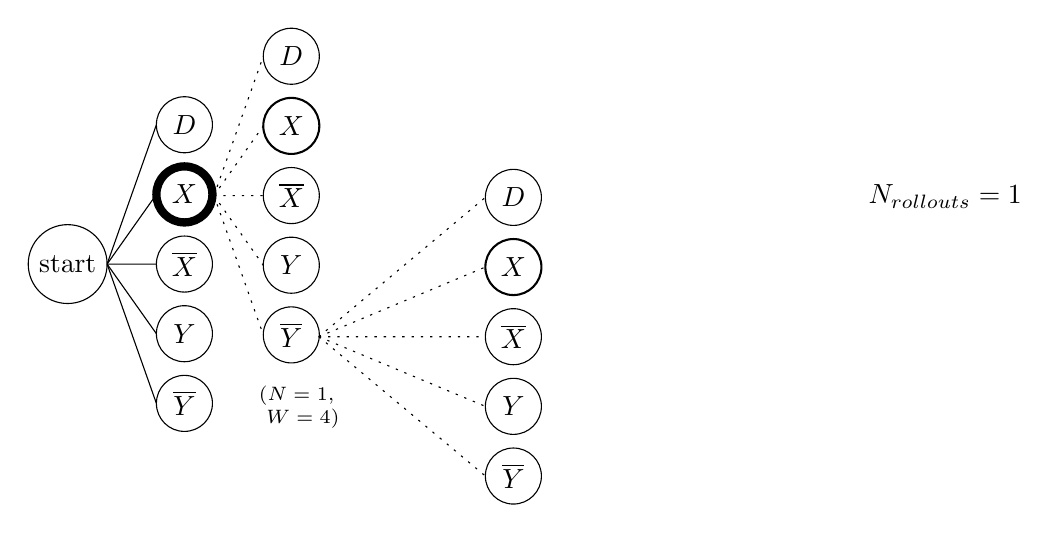
\begin{tikzpicture}[x=0.75pt,y=0.75pt,yscale=-1,xscale=1]
%uncomment if require: \path (0,383); %set diagram left start at 0, and has height of 383

%Straight Lines [id:da292697576636183] 
\draw    (74.5,208.63) -- (98.25,175.06) ;
%Shape: Circle [id:dp33372943337832695] 
\draw   (36.5,208.63) .. controls (36.5,198.13) and (45.01,189.63) .. (55.5,189.63) .. controls (65.99,189.63) and (74.5,198.13) .. (74.5,208.63) .. controls (74.5,219.12) and (65.99,227.63) .. (55.5,227.63) .. controls (45.01,227.63) and (36.5,219.12) .. (36.5,208.63) -- cycle ;

%Shape: Circle [id:dp9797672635345271] 
\draw   (98.25,141.5) .. controls (98.25,134.04) and (104.29,128) .. (111.75,128) .. controls (119.21,128) and (125.25,134.04) .. (125.25,141.5) .. controls (125.25,148.96) and (119.21,155) .. (111.75,155) .. controls (104.29,155) and (98.25,148.96) .. (98.25,141.5) -- cycle ;

%Shape: Circle [id:dp8614702115198233] 
\draw  [line width=3]  (98.25,175.06) .. controls (98.25,167.6) and (104.29,161.56) .. (111.75,161.56) .. controls (119.21,161.56) and (125.25,167.6) .. (125.25,175.06) .. controls (125.25,182.52) and (119.21,188.56) .. (111.75,188.56) .. controls (104.29,188.56) and (98.25,182.52) .. (98.25,175.06) -- cycle ;

%Shape: Circle [id:dp1575676913033387] 
\draw   (98.25,208.62) .. controls (98.25,201.16) and (104.29,195.12) .. (111.75,195.12) .. controls (119.21,195.12) and (125.25,201.16) .. (125.25,208.62) .. controls (125.25,216.08) and (119.21,222.12) .. (111.75,222.12) .. controls (104.29,222.12) and (98.25,216.08) .. (98.25,208.62) -- cycle ;

%Shape: Circle [id:dp05225998970447321] 
\draw   (98.25,275.75) .. controls (98.25,268.29) and (104.29,262.25) .. (111.75,262.25) .. controls (119.21,262.25) and (125.25,268.29) .. (125.25,275.75) .. controls (125.25,283.21) and (119.21,289.25) .. (111.75,289.25) .. controls (104.29,289.25) and (98.25,283.21) .. (98.25,275.75) -- cycle ;

%Shape: Circle [id:dp05391872355562477] 
\draw   (98.25,242.18) .. controls (98.25,234.72) and (104.29,228.68) .. (111.75,228.68) .. controls (119.21,228.68) and (125.25,234.72) .. (125.25,242.18) .. controls (125.25,249.64) and (119.21,255.68) .. (111.75,255.68) .. controls (104.29,255.68) and (98.25,249.64) .. (98.25,242.18) -- cycle ;

%Straight Lines [id:da15732371472419993] 
\draw    (74.5,208.63) -- (98.25,208.62) ;
%Straight Lines [id:da5265521885860803] 
\draw    (74.5,208.63) -- (98.25,141.5) ;
%Straight Lines [id:da4632869034305661] 
\draw    (74.5,208.63) -- (98.25,242.18) ;
%Straight Lines [id:da08854061217113685] 
\draw    (74.5,208.63) -- (98.25,275.75) ;
%Straight Lines [id:da6454559832471456] 
\draw  [dash pattern={on 0.84pt off 2.51pt}]  (126,175.63) -- (149.75,142.06) ;
%Shape: Circle [id:dp6998862923108375] 
\draw   (149.75,108.5) .. controls (149.75,101.04) and (155.79,95) .. (163.25,95) .. controls (170.71,95) and (176.75,101.04) .. (176.75,108.5) .. controls (176.75,115.96) and (170.71,122) .. (163.25,122) .. controls (155.79,122) and (149.75,115.96) .. (149.75,108.5) -- cycle ;

%Shape: Circle [id:dp7556655332713305] 
\draw  [line width=0.75]  (149.75,142.06) .. controls (149.75,134.6) and (155.79,128.56) .. (163.25,128.56) .. controls (170.71,128.56) and (176.75,134.6) .. (176.75,142.06) .. controls (176.75,149.52) and (170.71,155.56) .. (163.25,155.56) .. controls (155.79,155.56) and (149.75,149.52) .. (149.75,142.06) -- cycle ;

%Shape: Circle [id:dp5930768677610962] 
\draw   (149.75,175.62) .. controls (149.75,168.16) and (155.79,162.12) .. (163.25,162.12) .. controls (170.71,162.12) and (176.75,168.16) .. (176.75,175.62) .. controls (176.75,183.08) and (170.71,189.12) .. (163.25,189.12) .. controls (155.79,189.12) and (149.75,183.08) .. (149.75,175.62) -- cycle ;

%Shape: Circle [id:dp8190423265266639] 
\draw   (149.75,242.75) .. controls (149.75,235.29) and (155.79,229.25) .. (163.25,229.25) .. controls (170.71,229.25) and (176.75,235.29) .. (176.75,242.75) .. controls (176.75,250.21) and (170.71,256.25) .. (163.25,256.25) .. controls (155.79,256.25) and (149.75,250.21) .. (149.75,242.75) -- cycle ;

%Shape: Circle [id:dp8580534122132831] 
\draw   (149.75,209.18) .. controls (149.75,201.72) and (155.79,195.68) .. (163.25,195.68) .. controls (170.71,195.68) and (176.75,201.72) .. (176.75,209.18) .. controls (176.75,216.64) and (170.71,222.68) .. (163.25,222.68) .. controls (155.79,222.68) and (149.75,216.64) .. (149.75,209.18) -- cycle ;

%Straight Lines [id:da07498894986602467] 
\draw  [dash pattern={on 0.84pt off 2.51pt}]  (126,175.63) -- (149.75,175.62) ;
%Straight Lines [id:da844035584285212] 
\draw  [dash pattern={on 0.84pt off 2.51pt}]  (126,175.63) -- (149.75,108.5) ;
%Straight Lines [id:da6818354033246236] 
\draw  [dash pattern={on 0.84pt off 2.51pt}]  (126,175.63) -- (149.75,209.18) ;
%Straight Lines [id:da5698204535311175] 
\draw  [dash pattern={on 0.84pt off 2.51pt}]  (126,175.63) -- (149.75,242.75) ;

%Straight Lines [id:da8632677825172185] 
\draw  [dash pattern={on 0.84pt off 2.51pt}]  (176.5,243.63) -- (256.75,210.06) ;
%Shape: Circle [id:dp7216207520099238] 
\draw   (256.75,176.5) .. controls (256.75,169.04) and (262.79,163) .. (270.25,163) .. controls (277.71,163) and (283.75,169.04) .. (283.75,176.5) .. controls (283.75,183.96) and (277.71,190) .. (270.25,190) .. controls (262.79,190) and (256.75,183.96) .. (256.75,176.5) -- cycle ;

%Shape: Circle [id:dp3799879754651534] 
\draw  [line width=0.75]  (256.75,210.06) .. controls (256.75,202.6) and (262.79,196.56) .. (270.25,196.56) .. controls (277.71,196.56) and (283.75,202.6) .. (283.75,210.06) .. controls (283.75,217.52) and (277.71,223.56) .. (270.25,223.56) .. controls (262.79,223.56) and (256.75,217.52) .. (256.75,210.06) -- cycle ;

%Shape: Circle [id:dp8443813085322884] 
\draw   (256.75,243.62) .. controls (256.75,236.16) and (262.79,230.12) .. (270.25,230.12) .. controls (277.71,230.12) and (283.75,236.16) .. (283.75,243.62) .. controls (283.75,251.08) and (277.71,257.12) .. (270.25,257.12) .. controls (262.79,257.12) and (256.75,251.08) .. (256.75,243.62) -- cycle ;

%Shape: Circle [id:dp7261412171051816] 
\draw   (256.75,310.75) .. controls (256.75,303.29) and (262.79,297.25) .. (270.25,297.25) .. controls (277.71,297.25) and (283.75,303.29) .. (283.75,310.75) .. controls (283.75,318.21) and (277.71,324.25) .. (270.25,324.25) .. controls (262.79,324.25) and (256.75,318.21) .. (256.75,310.75) -- cycle ;

%Shape: Circle [id:dp823820400788563] 
\draw   (256.75,277.18) .. controls (256.75,269.72) and (262.79,263.68) .. (270.25,263.68) .. controls (277.71,263.68) and (283.75,269.72) .. (283.75,277.18) .. controls (283.75,284.64) and (277.71,290.68) .. (270.25,290.68) .. controls (262.79,290.68) and (256.75,284.64) .. (256.75,277.18) -- cycle ;

%Straight Lines [id:da5937383049004268] 
\draw  [dash pattern={on 0.84pt off 2.51pt}]  (176.5,243.63) -- (256.75,243.62) ;
%Straight Lines [id:da14325408869863376] 
\draw  [dash pattern={on 0.84pt off 2.51pt}]  (176.5,243.63) -- (256.75,176.5) ;
%Straight Lines [id:da7079350144706755] 
\draw  [dash pattern={on 0.84pt off 2.51pt}]  (176.5,243.63) -- (256.75,277.18) ;
%Straight Lines [id:da08427977647704898] 
\draw  [dash pattern={on 0.84pt off 2.51pt}]  (176.5,243.63) -- (256.75,310.75) ;


% Text Node
\draw (478.31,176.13) node  [font=\normalsize] [align=left] {$\displaystyle N_{\text{rollouts}} =1$};
% Text Node
\draw (270.25,277.18) node   [align=left] {$\displaystyle Y$};
% Text Node
\draw (270.25,310.75) node   [align=left] {$\displaystyle \overline{Y}$};
% Text Node
\draw (270.25,243.62) node   [align=left] {$\displaystyle \overline{X}$};
% Text Node
\draw (270.25,210.06) node   [align=left] {$\displaystyle X$};
% Text Node
\draw (270.25,176.5) node   [align=left] {$\displaystyle D$};
% Text Node
\draw (163.25,209.18) node   [align=left] {$\displaystyle Y$};
% Text Node
\draw (163.25,242.75) node   [align=left] {$\displaystyle \overline{Y}$};
% Text Node
\draw (163.25,175.62) node   [align=left] {$\displaystyle \overline{X}$};
% Text Node
\draw (163.25,142.06) node   [align=left] {$\displaystyle X$};
% Text Node
\draw (163.25,108.5) node   [align=left] {$\displaystyle D$};
% Text Node
\draw (111.75,242.18) node   [align=left] {$\displaystyle Y$};
% Text Node
\draw (111.75,275.75) node   [align=left] {$\displaystyle \overline{Y}$};
% Text Node
\draw (111.75,208.62) node   [align=left] {$\displaystyle \overline{X}$};
% Text Node
\draw (111.75,175.06) node   [align=left] {$\displaystyle X$};
% Text Node
\draw (111.75,141.5) node   [align=left] {$\displaystyle D$};
% Text Node
\draw (55.5,208.63) node   [align=left] {start};
% Text Node
\draw (167.04,277.78) node  [font=\scriptsize] [align=left] {$\displaystyle  \begin{array}{{>{\displaystyle}l}}
( N=1,\\
\ W=4)
\end{array}$};


\end{tikzpicture}

}
\end{figure}

\begin{figure}
\centering
\scalebox{.6}{
\input{../tikz/MCTS/MCTS-4.txt}
}
\end{figure}

\begin{figure}
\centering
\scalebox{.6}{


\tikzset{every picture/.style={line width=0.75pt}} %set default line width to 0.75pt        

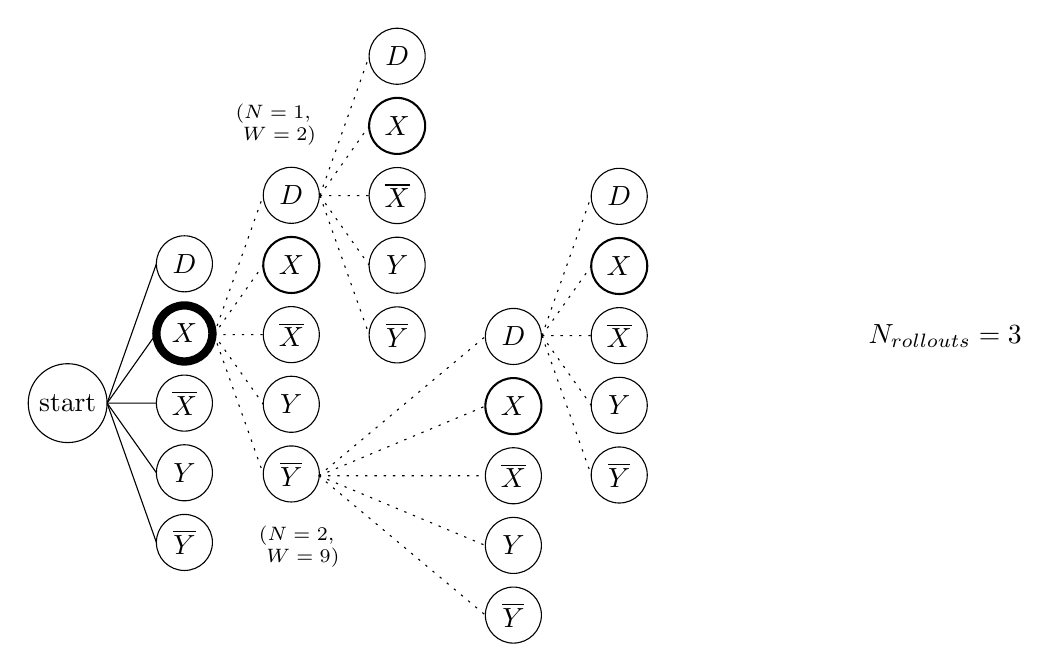
\begin{tikzpicture}[x=0.75pt,y=0.75pt,yscale=-1,xscale=1]
%uncomment if require: \path (0,383); %set diagram left start at 0, and has height of 383

%Straight Lines [id:da292697576636183] 
\draw    (74.5,208.63) -- (98.25,175.06) ;
%Shape: Circle [id:dp33372943337832695] 
\draw   (36.5,208.63) .. controls (36.5,198.13) and (45.01,189.63) .. (55.5,189.63) .. controls (65.99,189.63) and (74.5,198.13) .. (74.5,208.63) .. controls (74.5,219.12) and (65.99,227.63) .. (55.5,227.63) .. controls (45.01,227.63) and (36.5,219.12) .. (36.5,208.63) -- cycle ;

%Shape: Circle [id:dp9797672635345271] 
\draw   (98.25,141.5) .. controls (98.25,134.04) and (104.29,128) .. (111.75,128) .. controls (119.21,128) and (125.25,134.04) .. (125.25,141.5) .. controls (125.25,148.96) and (119.21,155) .. (111.75,155) .. controls (104.29,155) and (98.25,148.96) .. (98.25,141.5) -- cycle ;

%Shape: Circle [id:dp8614702115198233] 
\draw  [line width=3]  (98.25,175.06) .. controls (98.25,167.6) and (104.29,161.56) .. (111.75,161.56) .. controls (119.21,161.56) and (125.25,167.6) .. (125.25,175.06) .. controls (125.25,182.52) and (119.21,188.56) .. (111.75,188.56) .. controls (104.29,188.56) and (98.25,182.52) .. (98.25,175.06) -- cycle ;

%Shape: Circle [id:dp1575676913033387] 
\draw   (98.25,208.62) .. controls (98.25,201.16) and (104.29,195.12) .. (111.75,195.12) .. controls (119.21,195.12) and (125.25,201.16) .. (125.25,208.62) .. controls (125.25,216.08) and (119.21,222.12) .. (111.75,222.12) .. controls (104.29,222.12) and (98.25,216.08) .. (98.25,208.62) -- cycle ;

%Shape: Circle [id:dp05225998970447321] 
\draw   (98.25,275.75) .. controls (98.25,268.29) and (104.29,262.25) .. (111.75,262.25) .. controls (119.21,262.25) and (125.25,268.29) .. (125.25,275.75) .. controls (125.25,283.21) and (119.21,289.25) .. (111.75,289.25) .. controls (104.29,289.25) and (98.25,283.21) .. (98.25,275.75) -- cycle ;

%Shape: Circle [id:dp05391872355562477] 
\draw   (98.25,242.18) .. controls (98.25,234.72) and (104.29,228.68) .. (111.75,228.68) .. controls (119.21,228.68) and (125.25,234.72) .. (125.25,242.18) .. controls (125.25,249.64) and (119.21,255.68) .. (111.75,255.68) .. controls (104.29,255.68) and (98.25,249.64) .. (98.25,242.18) -- cycle ;

%Straight Lines [id:da15732371472419993] 
\draw    (74.5,208.63) -- (98.25,208.62) ;
%Straight Lines [id:da5265521885860803] 
\draw    (74.5,208.63) -- (98.25,141.5) ;
%Straight Lines [id:da4632869034305661] 
\draw    (74.5,208.63) -- (98.25,242.18) ;
%Straight Lines [id:da08854061217113685] 
\draw    (74.5,208.63) -- (98.25,275.75) ;
%Straight Lines [id:da6454559832471456] 
\draw  [dash pattern={on 0.84pt off 2.51pt}]  (126,175.63) -- (149.75,142.06) ;
%Shape: Circle [id:dp6998862923108375] 
\draw   (149.75,108.5) .. controls (149.75,101.04) and (155.79,95) .. (163.25,95) .. controls (170.71,95) and (176.75,101.04) .. (176.75,108.5) .. controls (176.75,115.96) and (170.71,122) .. (163.25,122) .. controls (155.79,122) and (149.75,115.96) .. (149.75,108.5) -- cycle ;

%Shape: Circle [id:dp7556655332713305] 
\draw  [line width=0.75]  (149.75,142.06) .. controls (149.75,134.6) and (155.79,128.56) .. (163.25,128.56) .. controls (170.71,128.56) and (176.75,134.6) .. (176.75,142.06) .. controls (176.75,149.52) and (170.71,155.56) .. (163.25,155.56) .. controls (155.79,155.56) and (149.75,149.52) .. (149.75,142.06) -- cycle ;

%Shape: Circle [id:dp5930768677610962] 
\draw   (149.75,175.62) .. controls (149.75,168.16) and (155.79,162.12) .. (163.25,162.12) .. controls (170.71,162.12) and (176.75,168.16) .. (176.75,175.62) .. controls (176.75,183.08) and (170.71,189.12) .. (163.25,189.12) .. controls (155.79,189.12) and (149.75,183.08) .. (149.75,175.62) -- cycle ;

%Shape: Circle [id:dp8190423265266639] 
\draw   (149.75,242.75) .. controls (149.75,235.29) and (155.79,229.25) .. (163.25,229.25) .. controls (170.71,229.25) and (176.75,235.29) .. (176.75,242.75) .. controls (176.75,250.21) and (170.71,256.25) .. (163.25,256.25) .. controls (155.79,256.25) and (149.75,250.21) .. (149.75,242.75) -- cycle ;

%Shape: Circle [id:dp8580534122132831] 
\draw   (149.75,209.18) .. controls (149.75,201.72) and (155.79,195.68) .. (163.25,195.68) .. controls (170.71,195.68) and (176.75,201.72) .. (176.75,209.18) .. controls (176.75,216.64) and (170.71,222.68) .. (163.25,222.68) .. controls (155.79,222.68) and (149.75,216.64) .. (149.75,209.18) -- cycle ;

%Straight Lines [id:da07498894986602467] 
\draw  [dash pattern={on 0.84pt off 2.51pt}]  (126,175.63) -- (149.75,175.62) ;
%Straight Lines [id:da844035584285212] 
\draw  [dash pattern={on 0.84pt off 2.51pt}]  (126,175.63) -- (149.75,108.5) ;
%Straight Lines [id:da6818354033246236] 
\draw  [dash pattern={on 0.84pt off 2.51pt}]  (126,175.63) -- (149.75,209.18) ;
%Straight Lines [id:da5698204535311175] 
\draw  [dash pattern={on 0.84pt off 2.51pt}]  (126,175.63) -- (149.75,242.75) ;

%Straight Lines [id:da6030853366529921] 
\draw  [dash pattern={on 0.84pt off 2.51pt}]  (284,176.13) -- (307.75,142.56) ;
%Shape: Circle [id:dp592877715644665] 
\draw   (307.75,109) .. controls (307.75,101.54) and (313.79,95.5) .. (321.25,95.5) .. controls (328.71,95.5) and (334.75,101.54) .. (334.75,109) .. controls (334.75,116.46) and (328.71,122.5) .. (321.25,122.5) .. controls (313.79,122.5) and (307.75,116.46) .. (307.75,109) -- cycle ;

%Shape: Circle [id:dp814364580188803] 
\draw  [line width=0.75]  (307.75,142.56) .. controls (307.75,135.1) and (313.79,129.06) .. (321.25,129.06) .. controls (328.71,129.06) and (334.75,135.1) .. (334.75,142.56) .. controls (334.75,150.02) and (328.71,156.06) .. (321.25,156.06) .. controls (313.79,156.06) and (307.75,150.02) .. (307.75,142.56) -- cycle ;

%Shape: Circle [id:dp7433809978898483] 
\draw   (307.75,176.12) .. controls (307.75,168.66) and (313.79,162.62) .. (321.25,162.62) .. controls (328.71,162.62) and (334.75,168.66) .. (334.75,176.12) .. controls (334.75,183.58) and (328.71,189.62) .. (321.25,189.62) .. controls (313.79,189.62) and (307.75,183.58) .. (307.75,176.12) -- cycle ;

%Shape: Circle [id:dp9104599451042091] 
\draw   (307.75,243.25) .. controls (307.75,235.79) and (313.79,229.75) .. (321.25,229.75) .. controls (328.71,229.75) and (334.75,235.79) .. (334.75,243.25) .. controls (334.75,250.71) and (328.71,256.75) .. (321.25,256.75) .. controls (313.79,256.75) and (307.75,250.71) .. (307.75,243.25) -- cycle ;

%Shape: Circle [id:dp32102708796117985] 
\draw   (307.75,209.68) .. controls (307.75,202.22) and (313.79,196.18) .. (321.25,196.18) .. controls (328.71,196.18) and (334.75,202.22) .. (334.75,209.68) .. controls (334.75,217.14) and (328.71,223.18) .. (321.25,223.18) .. controls (313.79,223.18) and (307.75,217.14) .. (307.75,209.68) -- cycle ;

%Straight Lines [id:da48939229833818054] 
\draw  [dash pattern={on 0.84pt off 2.51pt}]  (284,176.13) -- (307.75,176.12) ;
%Straight Lines [id:da9348134303007142] 
\draw  [dash pattern={on 0.84pt off 2.51pt}]  (284,176.13) -- (307.75,109) ;
%Straight Lines [id:da5635356286228058] 
\draw  [dash pattern={on 0.84pt off 2.51pt}]  (284,176.13) -- (307.75,209.68) ;
%Straight Lines [id:da3342222050871244] 
\draw  [dash pattern={on 0.84pt off 2.51pt}]  (284,176.13) -- (307.75,243.25) ;

%Straight Lines [id:da8632677825172185] 
\draw  [dash pattern={on 0.84pt off 2.51pt}]  (176.5,243.63) -- (256.75,210.06) ;
%Shape: Circle [id:dp7216207520099238] 
\draw   (256.75,176.5) .. controls (256.75,169.04) and (262.79,163) .. (270.25,163) .. controls (277.71,163) and (283.75,169.04) .. (283.75,176.5) .. controls (283.75,183.96) and (277.71,190) .. (270.25,190) .. controls (262.79,190) and (256.75,183.96) .. (256.75,176.5) -- cycle ;

%Shape: Circle [id:dp3799879754651534] 
\draw  [line width=0.75]  (256.75,210.06) .. controls (256.75,202.6) and (262.79,196.56) .. (270.25,196.56) .. controls (277.71,196.56) and (283.75,202.6) .. (283.75,210.06) .. controls (283.75,217.52) and (277.71,223.56) .. (270.25,223.56) .. controls (262.79,223.56) and (256.75,217.52) .. (256.75,210.06) -- cycle ;

%Shape: Circle [id:dp8443813085322884] 
\draw   (256.75,243.62) .. controls (256.75,236.16) and (262.79,230.12) .. (270.25,230.12) .. controls (277.71,230.12) and (283.75,236.16) .. (283.75,243.62) .. controls (283.75,251.08) and (277.71,257.12) .. (270.25,257.12) .. controls (262.79,257.12) and (256.75,251.08) .. (256.75,243.62) -- cycle ;

%Shape: Circle [id:dp7261412171051816] 
\draw   (256.75,310.75) .. controls (256.75,303.29) and (262.79,297.25) .. (270.25,297.25) .. controls (277.71,297.25) and (283.75,303.29) .. (283.75,310.75) .. controls (283.75,318.21) and (277.71,324.25) .. (270.25,324.25) .. controls (262.79,324.25) and (256.75,318.21) .. (256.75,310.75) -- cycle ;

%Shape: Circle [id:dp823820400788563] 
\draw   (256.75,277.18) .. controls (256.75,269.72) and (262.79,263.68) .. (270.25,263.68) .. controls (277.71,263.68) and (283.75,269.72) .. (283.75,277.18) .. controls (283.75,284.64) and (277.71,290.68) .. (270.25,290.68) .. controls (262.79,290.68) and (256.75,284.64) .. (256.75,277.18) -- cycle ;

%Straight Lines [id:da5937383049004268] 
\draw  [dash pattern={on 0.84pt off 2.51pt}]  (176.5,243.63) -- (256.75,243.62) ;
%Straight Lines [id:da14325408869863376] 
\draw  [dash pattern={on 0.84pt off 2.51pt}]  (176.5,243.63) -- (256.75,176.5) ;
%Straight Lines [id:da7079350144706755] 
\draw  [dash pattern={on 0.84pt off 2.51pt}]  (176.5,243.63) -- (256.75,277.18) ;
%Straight Lines [id:da08427977647704898] 
\draw  [dash pattern={on 0.84pt off 2.51pt}]  (176.5,243.63) -- (256.75,310.75) ;

%Straight Lines [id:da9650022346312773] 
\draw  [dash pattern={on 0.84pt off 2.51pt}]  (177,108.63) -- (200.75,75.06) ;
%Shape: Circle [id:dp5672483495136048] 
\draw   (200.75,41.5) .. controls (200.75,34.04) and (206.79,28) .. (214.25,28) .. controls (221.71,28) and (227.75,34.04) .. (227.75,41.5) .. controls (227.75,48.96) and (221.71,55) .. (214.25,55) .. controls (206.79,55) and (200.75,48.96) .. (200.75,41.5) -- cycle ;

%Shape: Circle [id:dp6259967501394085] 
\draw  [line width=0.75]  (200.75,75.06) .. controls (200.75,67.6) and (206.79,61.56) .. (214.25,61.56) .. controls (221.71,61.56) and (227.75,67.6) .. (227.75,75.06) .. controls (227.75,82.52) and (221.71,88.56) .. (214.25,88.56) .. controls (206.79,88.56) and (200.75,82.52) .. (200.75,75.06) -- cycle ;

%Shape: Circle [id:dp8641975762213093] 
\draw   (200.75,108.62) .. controls (200.75,101.16) and (206.79,95.12) .. (214.25,95.12) .. controls (221.71,95.12) and (227.75,101.16) .. (227.75,108.62) .. controls (227.75,116.08) and (221.71,122.12) .. (214.25,122.12) .. controls (206.79,122.12) and (200.75,116.08) .. (200.75,108.62) -- cycle ;

%Shape: Circle [id:dp27955532063236155] 
\draw   (200.75,175.75) .. controls (200.75,168.29) and (206.79,162.25) .. (214.25,162.25) .. controls (221.71,162.25) and (227.75,168.29) .. (227.75,175.75) .. controls (227.75,183.21) and (221.71,189.25) .. (214.25,189.25) .. controls (206.79,189.25) and (200.75,183.21) .. (200.75,175.75) -- cycle ;

%Shape: Circle [id:dp6604261332787644] 
\draw   (200.75,142.18) .. controls (200.75,134.72) and (206.79,128.68) .. (214.25,128.68) .. controls (221.71,128.68) and (227.75,134.72) .. (227.75,142.18) .. controls (227.75,149.64) and (221.71,155.68) .. (214.25,155.68) .. controls (206.79,155.68) and (200.75,149.64) .. (200.75,142.18) -- cycle ;

%Straight Lines [id:da46297939376412267] 
\draw  [dash pattern={on 0.84pt off 2.51pt}]  (177,108.63) -- (200.75,108.62) ;
%Straight Lines [id:da34734619250993637] 
\draw  [dash pattern={on 0.84pt off 2.51pt}]  (177,108.63) -- (200.75,41.5) ;
%Straight Lines [id:da25630373805357953] 
\draw  [dash pattern={on 0.84pt off 2.51pt}]  (177,108.63) -- (200.75,142.18) ;
%Straight Lines [id:da8658108010043505] 
\draw  [dash pattern={on 0.84pt off 2.51pt}]  (177,108.63) -- (200.75,175.75) ;


% Text Node
\draw (478.31,176.13) node  [font=\normalsize] [align=left] {$\displaystyle N_{\text{rollouts}} =3$};
% Text Node
\draw (214.25,142.18) node   [align=left] {$\displaystyle Y$};
% Text Node
\draw (214.25,175.75) node   [align=left] {$\displaystyle \overline{Y}$};
% Text Node
\draw (214.25,108.62) node   [align=left] {$\displaystyle \overline{X}$};
% Text Node
\draw (214.25,75.06) node   [align=left] {$\displaystyle X$};
% Text Node
\draw (214.25,41.5) node   [align=left] {$\displaystyle D$};
% Text Node
\draw (270.25,277.18) node   [align=left] {$\displaystyle Y$};
% Text Node
\draw (270.25,310.75) node   [align=left] {$\displaystyle \overline{Y}$};
% Text Node
\draw (270.25,243.62) node   [align=left] {$\displaystyle \overline{X}$};
% Text Node
\draw (270.25,210.06) node   [align=left] {$\displaystyle X$};
% Text Node
\draw (270.25,176.5) node   [align=left] {$\displaystyle D$};
% Text Node
\draw (321.25,209.68) node   [align=left] {$\displaystyle Y$};
% Text Node
\draw (321.25,243.25) node   [align=left] {$\displaystyle \overline{Y}$};
% Text Node
\draw (321.25,176.12) node   [align=left] {$\displaystyle \overline{X}$};
% Text Node
\draw (321.25,142.56) node   [align=left] {$\displaystyle X$};
% Text Node
\draw (321.25,109) node   [align=left] {$\displaystyle D$};
% Text Node
\draw (163.25,209.18) node   [align=left] {$\displaystyle Y$};
% Text Node
\draw (163.25,242.75) node   [align=left] {$\displaystyle \overline{Y}$};
% Text Node
\draw (163.25,175.62) node   [align=left] {$\displaystyle \overline{X}$};
% Text Node
\draw (163.25,142.06) node   [align=left] {$\displaystyle X$};
% Text Node
\draw (163.25,108.5) node   [align=left] {$\displaystyle D$};
% Text Node
\draw (111.75,242.18) node   [align=left] {$\displaystyle Y$};
% Text Node
\draw (111.75,275.75) node   [align=left] {$\displaystyle \overline{Y}$};
% Text Node
\draw (111.75,208.62) node   [align=left] {$\displaystyle \overline{X}$};
% Text Node
\draw (111.75,175.06) node   [align=left] {$\displaystyle X$};
% Text Node
\draw (111.75,141.5) node   [align=left] {$\displaystyle D$};
% Text Node
\draw (55.5,208.63) node   [align=left] {start};
% Text Node
\draw (167.04,277.78) node  [font=\scriptsize] [align=left] {$\displaystyle  \begin{array}{{>{\displaystyle}l}}
( N=2,\\
\ W=9)
\end{array}$};
% Text Node
\draw (155.78,74.78) node  [font=\scriptsize] [align=left] {$\displaystyle  \begin{array}{{>{\displaystyle}l}}
( N=1,\\
\ W=2)
\end{array}$};


\end{tikzpicture}

}
\end{figure}



\end{frame}



\begin{frame}{AlphaZero: network training}

Pulse sequence data comes in from MCTS\dots

    \begin{figure}
    \centering
    \scalebox{.6}{
    

\tikzset{every picture/.style={line width=0.75pt}} %set default line width to 0.75pt

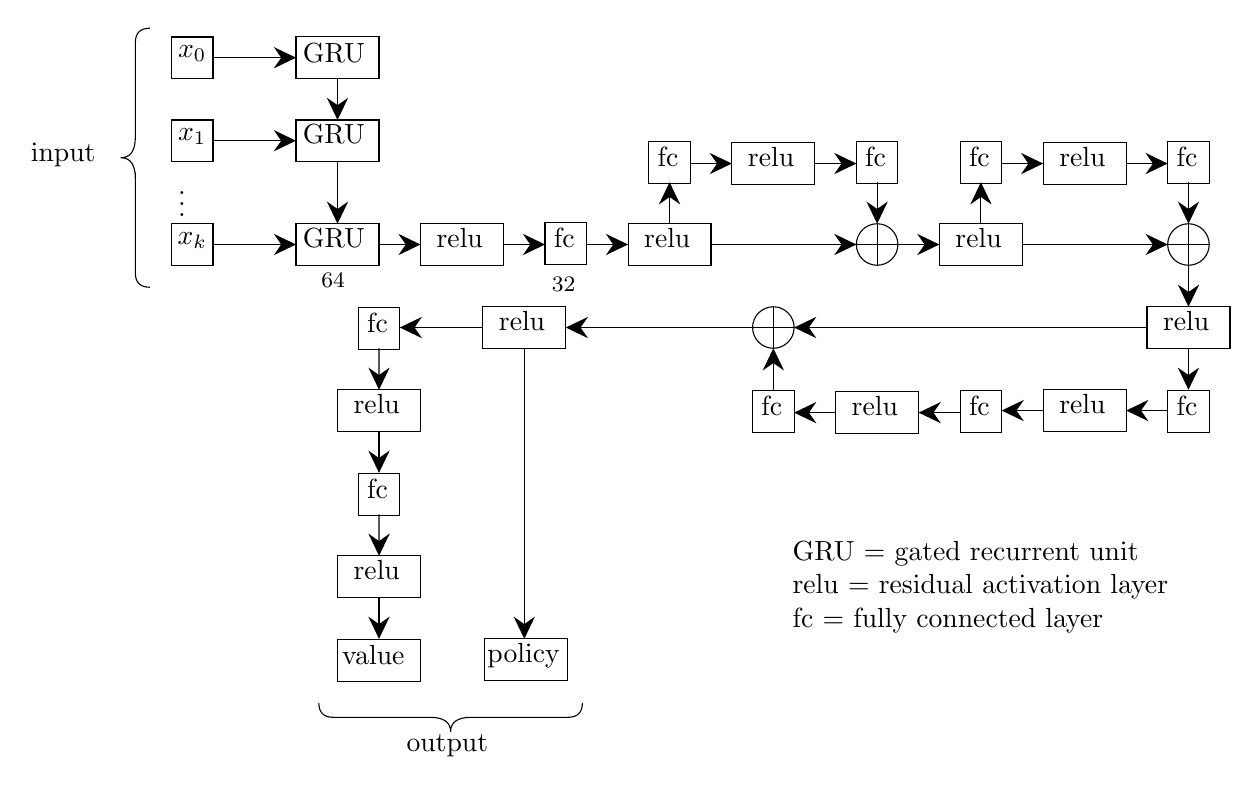
\begin{tikzpicture}[x=0.75pt,y=0.75pt,yscale=-1,xscale=1]
%uncomment if require: \path (0,382); %set diagram left start at 0, and has height of 382

%Shape: Rectangle [id:dp02638136849538708]
\draw   (90.01,20.25) -- (110.01,20.25) -- (110.01,40.25) -- (90.01,40.25) -- cycle ;
%Shape: Rectangle [id:dp4204285901048066]
\draw   (90,60.2) -- (110,60.2) -- (110,80.2) -- (90,80.2) -- cycle ;
%Straight Lines [id:da18786128196874485]
\draw    (110.02,30.2) -- (147.02,30.2) ;
\draw [shift={(150.02,30.2)}, rotate = 180] [fill={rgb, 255:red, 0; green, 0; blue, 0 }  ][line width=0.08]  [draw opacity=0] (10.72,-5.15) -- (0,0) -- (10.72,5.15) -- (7.12,0) -- cycle    ;
%Straight Lines [id:da8836932503131412]
\draw    (110.01,70.2) -- (147.01,70.2) ;
\draw [shift={(150.01,70.2)}, rotate = 180] [fill={rgb, 255:red, 0; green, 0; blue, 0 }  ][line width=0.08]  [draw opacity=0] (10.72,-5.15) -- (0,0) -- (10.72,5.15) -- (7.12,0) -- cycle    ;
%Straight Lines [id:da3922749523317497]
\draw    (170.02,40.2) -- (170.02,57.2) ;
\draw [shift={(170.02,60.2)}, rotate = 270] [fill={rgb, 255:red, 0; green, 0; blue, 0 }  ][line width=0.08]  [draw opacity=0] (10.72,-5.15) -- (0,0) -- (10.72,5.15) -- (7.12,0) -- cycle    ;
%Shape: Rectangle [id:dp32409815423962685]
\draw   (150.02,20.2) -- (190.02,20.2) -- (190.02,40.2) -- (150.02,40.2) -- cycle ;
%Shape: Rectangle [id:dp7239061253067598]
\draw   (150.01,60.2) -- (190.01,60.2) -- (190.01,80.2) -- (150.01,80.2) -- cycle ;
%Shape: Rectangle [id:dp7205034746760461]
\draw   (90.01,110.2) -- (110.01,110.2) -- (110.01,130.2) -- (90.01,130.2) -- cycle ;
%Straight Lines [id:da2768291231406834]
\draw    (110.02,120.2) -- (147.02,120.2) ;
\draw [shift={(150.02,120.2)}, rotate = 180] [fill={rgb, 255:red, 0; green, 0; blue, 0 }  ][line width=0.08]  [draw opacity=0] (10.72,-5.15) -- (0,0) -- (10.72,5.15) -- (7.12,0) -- cycle    ;
%Straight Lines [id:da04420279990164899]
\draw    (170.02,80.2) -- (170.02,107.2) ;
\draw [shift={(170.02,110.2)}, rotate = 270] [fill={rgb, 255:red, 0; green, 0; blue, 0 }  ][line width=0.08]  [draw opacity=0] (10.72,-5.15) -- (0,0) -- (10.72,5.15) -- (7.12,0) -- cycle    ;
%Shape: Rectangle [id:dp5376553256891963]
\draw   (150.02,110.2) -- (190.02,110.2) -- (190.02,130.2) -- (150.02,130.2) -- cycle ;
%Shape: Rectangle [id:dp20156185382495795]
\draw   (210.02,110.2) -- (250,110.2) -- (250,130.2) -- (210.02,130.2) -- cycle ;
%Straight Lines [id:da792263985693916]
\draw    (190.02,120.2) -- (207.02,120.2) ;
\draw [shift={(210.02,120.2)}, rotate = 180] [fill={rgb, 255:red, 0; green, 0; blue, 0 }  ][line width=0.08]  [draw opacity=0] (10.72,-5.15) -- (0,0) -- (10.72,5.15) -- (7.12,0) -- cycle    ;
%Straight Lines [id:da6470713620273096]
\draw    (430,90.2) -- (430,107.2) ;
\draw [shift={(430,110.2)}, rotate = 270] [fill={rgb, 255:red, 0; green, 0; blue, 0 }  ][line width=0.08]  [draw opacity=0] (10.72,-5.15) -- (0,0) -- (10.72,5.15) -- (7.12,0) -- cycle    ;
%Flowchart: Or [id:dp6599768898399976]
\draw   (420,120.2) .. controls (420,114.68) and (424.48,110.2) .. (430,110.2) .. controls (435.52,110.2) and (440,114.68) .. (440,120.2) .. controls (440,125.72) and (435.52,130.2) .. (430,130.2) .. controls (424.48,130.2) and (420,125.72) .. (420,120.2) -- cycle ; \draw   (420,120.2) -- (440,120.2) ; \draw   (430,110.2) -- (430,130.2) ;
%Shape: Rectangle [id:dp7585346138321025]
\draw   (270,109.7) -- (290,109.7) -- (290,129.7) -- (270,129.7) -- cycle ;
%Straight Lines [id:da5278108394530496]
\draw    (250,120.2) -- (267,120.2) ;
\draw [shift={(270,120.2)}, rotate = 180] [fill={rgb, 255:red, 0; green, 0; blue, 0 }  ][line width=0.08]  [draw opacity=0] (10.72,-5.15) -- (0,0) -- (10.72,5.15) -- (7.12,0) -- cycle    ;
%Shape: Rectangle [id:dp45637585865043273]
\draw   (310,110.2) -- (349.98,110.2) -- (349.98,130.2) -- (310,130.2) -- cycle ;
%Straight Lines [id:da015144151772794379]
\draw    (290,120.2) -- (307,120.2) ;
\draw [shift={(310,120.2)}, rotate = 180] [fill={rgb, 255:red, 0; green, 0; blue, 0 }  ][line width=0.08]  [draw opacity=0] (10.72,-5.15) -- (0,0) -- (10.72,5.15) -- (7.12,0) -- cycle    ;
%Shape: Rectangle [id:dp680216878775233]
\draw   (320,70.7) -- (340,70.7) -- (340,90.7) -- (320,90.7) -- cycle ;
%Shape: Rectangle [id:dp7310722650845467]
\draw   (360,71.2) -- (399.98,71.2) -- (399.98,91.2) -- (360,91.2) -- cycle ;
%Straight Lines [id:da476677827076349]
\draw    (340,81.2) -- (357,81.2) ;
\draw [shift={(360,81.2)}, rotate = 180] [fill={rgb, 255:red, 0; green, 0; blue, 0 }  ][line width=0.08]  [draw opacity=0] (10.72,-5.15) -- (0,0) -- (10.72,5.15) -- (7.12,0) -- cycle    ;
%Straight Lines [id:da9800517663487802]
\draw    (330,110.2) -- (330,93.2) ;
\draw [shift={(330,90.2)}, rotate = 450] [fill={rgb, 255:red, 0; green, 0; blue, 0 }  ][line width=0.08]  [draw opacity=0] (10.72,-5.15) -- (0,0) -- (10.72,5.15) -- (7.12,0) -- cycle    ;
%Shape: Rectangle [id:dp021057905114674424]
\draw   (420,70.7) -- (440,70.7) -- (440,90.7) -- (420,90.7) -- cycle ;
%Straight Lines [id:da19829953520297927]
\draw    (400,81.2) -- (417,81.2) ;
\draw [shift={(420,81.2)}, rotate = 180] [fill={rgb, 255:red, 0; green, 0; blue, 0 }  ][line width=0.08]  [draw opacity=0] (10.72,-5.15) -- (0,0) -- (10.72,5.15) -- (7.12,0) -- cycle    ;
%Straight Lines [id:da37662612388777994]
\draw    (350,120.2) -- (417,120.2) ;
\draw [shift={(420,120.2)}, rotate = 180] [fill={rgb, 255:red, 0; green, 0; blue, 0 }  ][line width=0.08]  [draw opacity=0] (10.72,-5.15) -- (0,0) -- (10.72,5.15) -- (7.12,0) -- cycle    ;
%Shape: Rectangle [id:dp5579644555480454]
\draw   (560.02,150.2) -- (600,150.2) -- (600,170.2) -- (560.02,170.2) -- cycle ;
%Straight Lines [id:da06494630042228744]
\draw    (580.02,130.2) -- (580.02,147.2) ;
\draw [shift={(580.02,150.2)}, rotate = 270] [fill={rgb, 255:red, 0; green, 0; blue, 0 }  ][line width=0.08]  [draw opacity=0] (10.72,-5.15) -- (0,0) -- (10.72,5.15) -- (7.12,0) -- cycle    ;
%Straight Lines [id:da8876672874205853]
\draw    (580,90.2) -- (580,107.2) ;
\draw [shift={(580,110.2)}, rotate = 270] [fill={rgb, 255:red, 0; green, 0; blue, 0 }  ][line width=0.08]  [draw opacity=0] (10.72,-5.15) -- (0,0) -- (10.72,5.15) -- (7.12,0) -- cycle    ;
%Flowchart: Or [id:dp7508932175580134]
\draw   (570,120.2) .. controls (570,114.68) and (574.48,110.2) .. (580,110.2) .. controls (585.52,110.2) and (590,114.68) .. (590,120.2) .. controls (590,125.72) and (585.52,130.2) .. (580,130.2) .. controls (574.48,130.2) and (570,125.72) .. (570,120.2) -- cycle ; \draw   (570,120.2) -- (590,120.2) ; \draw   (580,110.2) -- (580,130.2) ;
%Shape: Rectangle [id:dp49517683581388927]
\draw   (460,110.2) -- (499.98,110.2) -- (499.98,130.2) -- (460,130.2) -- cycle ;
%Straight Lines [id:da9885418731285747]
\draw    (440,120.2) -- (457,120.2) ;
\draw [shift={(460,120.2)}, rotate = 180] [fill={rgb, 255:red, 0; green, 0; blue, 0 }  ][line width=0.08]  [draw opacity=0] (10.72,-5.15) -- (0,0) -- (10.72,5.15) -- (7.12,0) -- cycle    ;
%Shape: Rectangle [id:dp7101148618833939]
\draw   (470,70.7) -- (490,70.7) -- (490,90.7) -- (470,90.7) -- cycle ;
%Shape: Rectangle [id:dp6761712905766428]
\draw   (510,71.2) -- (549.98,71.2) -- (549.98,91.2) -- (510,91.2) -- cycle ;
%Straight Lines [id:da7602138343769007]
\draw    (490,81.2) -- (507,81.2) ;
\draw [shift={(510,81.2)}, rotate = 180] [fill={rgb, 255:red, 0; green, 0; blue, 0 }  ][line width=0.08]  [draw opacity=0] (10.72,-5.15) -- (0,0) -- (10.72,5.15) -- (7.12,0) -- cycle    ;
%Straight Lines [id:da44997478868284935]
\draw    (480,110.2) -- (480,93.2) ;
\draw [shift={(480,90.2)}, rotate = 450] [fill={rgb, 255:red, 0; green, 0; blue, 0 }  ][line width=0.08]  [draw opacity=0] (10.72,-5.15) -- (0,0) -- (10.72,5.15) -- (7.12,0) -- cycle    ;
%Shape: Rectangle [id:dp8001219618459012]
\draw   (570,70.7) -- (590,70.7) -- (590,90.7) -- (570,90.7) -- cycle ;
%Straight Lines [id:da8191439427145315]
\draw    (550,81.2) -- (567,81.2) ;
\draw [shift={(570,81.2)}, rotate = 180] [fill={rgb, 255:red, 0; green, 0; blue, 0 }  ][line width=0.08]  [draw opacity=0] (10.72,-5.15) -- (0,0) -- (10.72,5.15) -- (7.12,0) -- cycle    ;
%Straight Lines [id:da9263282941037065]
\draw    (500,120.2) -- (567,120.2) ;
\draw [shift={(570,120.2)}, rotate = 180] [fill={rgb, 255:red, 0; green, 0; blue, 0 }  ][line width=0.08]  [draw opacity=0] (10.72,-5.15) -- (0,0) -- (10.72,5.15) -- (7.12,0) -- cycle    ;
%Straight Lines [id:da1317984498790985]
\draw    (580,170.2) -- (580,187.2) ;
\draw [shift={(580,190.2)}, rotate = 270] [fill={rgb, 255:red, 0; green, 0; blue, 0 }  ][line width=0.08]  [draw opacity=0] (10.72,-5.15) -- (0,0) -- (10.72,5.15) -- (7.12,0) -- cycle    ;
%Shape: Rectangle [id:dp19231745792682342]
\draw   (570,190.7) -- (590,190.7) -- (590,210.7) -- (570,210.7) -- cycle ;
%Shape: Rectangle [id:dp3661262539844976]
\draw   (510,190.2) -- (549.98,190.2) -- (549.98,210.2) -- (510,210.2) -- cycle ;
%Straight Lines [id:da46430121112477796]
\draw    (570,200.2) -- (553,200.2) ;
\draw [shift={(550,200.2)}, rotate = 360] [fill={rgb, 255:red, 0; green, 0; blue, 0 }  ][line width=0.08]  [draw opacity=0] (10.72,-5.15) -- (0,0) -- (10.72,5.15) -- (7.12,0) -- cycle    ;
%Shape: Rectangle [id:dp7015582656278725]
\draw   (470,190.7) -- (490,190.7) -- (490,210.7) -- (470,210.7) -- cycle ;
%Straight Lines [id:da6274160240081927]
\draw    (510,200.2) -- (493,200.2) ;
\draw [shift={(490,200.2)}, rotate = 360] [fill={rgb, 255:red, 0; green, 0; blue, 0 }  ][line width=0.08]  [draw opacity=0] (10.72,-5.15) -- (0,0) -- (10.72,5.15) -- (7.12,0) -- cycle    ;
%Shape: Rectangle [id:dp5757706276069112]
\draw   (410,191.2) -- (449.98,191.2) -- (449.98,211.2) -- (410,211.2) -- cycle ;
%Straight Lines [id:da877816695924893]
\draw    (470,201.2) -- (453,201.2) ;
\draw [shift={(450,201.2)}, rotate = 360] [fill={rgb, 255:red, 0; green, 0; blue, 0 }  ][line width=0.08]  [draw opacity=0] (10.72,-5.15) -- (0,0) -- (10.72,5.15) -- (7.12,0) -- cycle    ;
%Shape: Rectangle [id:dp9665386619854055]
\draw   (370,190.7) -- (390,190.7) -- (390,210.7) -- (370,210.7) -- cycle ;
%Straight Lines [id:da43350283631446174]
\draw    (410,201.2) -- (393,201.2) ;
\draw [shift={(390,201.2)}, rotate = 360] [fill={rgb, 255:red, 0; green, 0; blue, 0 }  ][line width=0.08]  [draw opacity=0] (10.72,-5.15) -- (0,0) -- (10.72,5.15) -- (7.12,0) -- cycle    ;
%Flowchart: Or [id:dp6555350236573219]
\draw   (370,160.2) .. controls (370,154.68) and (374.48,150.2) .. (380,150.2) .. controls (385.52,150.2) and (390,154.68) .. (390,160.2) .. controls (390,165.72) and (385.52,170.2) .. (380,170.2) .. controls (374.48,170.2) and (370,165.72) .. (370,160.2) -- cycle ; \draw   (370,160.2) -- (390,160.2) ; \draw   (380,150.2) -- (380,170.2) ;
%Straight Lines [id:da9538541164521721]
\draw    (560,160.2) -- (393,160.2) ;
\draw [shift={(390,160.2)}, rotate = 360] [fill={rgb, 255:red, 0; green, 0; blue, 0 }  ][line width=0.08]  [draw opacity=0] (10.72,-5.15) -- (0,0) -- (10.72,5.15) -- (7.12,0) -- cycle    ;
%Straight Lines [id:da10469597971614442]
\draw    (380,190.2) -- (380,173.2) ;
\draw [shift={(380,170.2)}, rotate = 450] [fill={rgb, 255:red, 0; green, 0; blue, 0 }  ][line width=0.08]  [draw opacity=0] (10.72,-5.15) -- (0,0) -- (10.72,5.15) -- (7.12,0) -- cycle    ;
%Shape: Rectangle [id:dp07415870480577125]
\draw   (240.02,150.2) -- (280,150.2) -- (280,170.2) -- (240.02,170.2) -- cycle ;
%Straight Lines [id:da857184847829574]
\draw    (370,160.2) -- (283,160.2) ;
\draw [shift={(280,160.2)}, rotate = 360] [fill={rgb, 255:red, 0; green, 0; blue, 0 }  ][line width=0.08]  [draw opacity=0] (10.72,-5.15) -- (0,0) -- (10.72,5.15) -- (7.12,0) -- cycle    ;
%Shape: Rectangle [id:dp7255363648906021]
\draw   (241.01,310.2) -- (280.99,310.2) -- (280.99,330.2) -- (241.01,330.2) -- cycle ;
%Straight Lines [id:da10818889394863507]
\draw    (260,170.2) -- (260,307.2) ;
\draw [shift={(260,310.2)}, rotate = 270] [fill={rgb, 255:red, 0; green, 0; blue, 0 }  ][line width=0.08]  [draw opacity=0] (10.72,-5.15) -- (0,0) -- (10.72,5.15) -- (7.12,0) -- cycle    ;
%Shape: Rectangle [id:dp8701695128090077]
\draw   (180,150.7) -- (200,150.7) -- (200,170.7) -- (180,170.7) -- cycle ;
%Straight Lines [id:da0015163063151002465]
\draw    (240,160.2) -- (203,160.2) ;
\draw [shift={(200,160.2)}, rotate = 360] [fill={rgb, 255:red, 0; green, 0; blue, 0 }  ][line width=0.08]  [draw opacity=0] (10.72,-5.15) -- (0,0) -- (10.72,5.15) -- (7.12,0) -- cycle    ;
%Shape: Rectangle [id:dp11711776574433075]
\draw   (170.02,190.2) -- (210,190.2) -- (210,210.2) -- (170.02,210.2) -- cycle ;
%Straight Lines [id:da909719887882497]
\draw    (190,170.2) -- (190.02,187.2) ;
\draw [shift={(190.02,190.2)}, rotate = 269.93] [fill={rgb, 255:red, 0; green, 0; blue, 0 }  ][line width=0.08]  [draw opacity=0] (10.72,-5.15) -- (0,0) -- (10.72,5.15) -- (7.12,0) -- cycle    ;
%Straight Lines [id:da057281968974082886]
\draw    (190,210.2) -- (190,227.2) ;
\draw [shift={(190,230.2)}, rotate = 270] [fill={rgb, 255:red, 0; green, 0; blue, 0 }  ][line width=0.08]  [draw opacity=0] (10.72,-5.15) -- (0,0) -- (10.72,5.15) -- (7.12,0) -- cycle    ;
%Shape: Rectangle [id:dp11366092940797157]
\draw   (180,230.7) -- (200,230.7) -- (200,250.7) -- (180,250.7) -- cycle ;
%Shape: Rectangle [id:dp7686918520673491]
\draw   (170.02,270.2) -- (210,270.2) -- (210,290.2) -- (170.02,290.2) -- cycle ;
%Straight Lines [id:da284359228138074]
\draw    (190,250.2) -- (190.02,267.2) ;
\draw [shift={(190.02,270.2)}, rotate = 269.93] [fill={rgb, 255:red, 0; green, 0; blue, 0 }  ][line width=0.08]  [draw opacity=0] (10.72,-5.15) -- (0,0) -- (10.72,5.15) -- (7.12,0) -- cycle    ;
%Straight Lines [id:da5969772278968581]
\draw    (190,290.2) -- (190,307.2) ;
\draw [shift={(190,310.2)}, rotate = 270] [fill={rgb, 255:red, 0; green, 0; blue, 0 }  ][line width=0.08]  [draw opacity=0] (10.72,-5.15) -- (0,0) -- (10.72,5.15) -- (7.12,0) -- cycle    ;
%Shape: Rectangle [id:dp6607557330878455]
\draw   (170,310.7) -- (210,310.7) -- (210,330.7) -- (170,330.7) -- cycle ;
%Shape: Brace [id:dp14557160899369648]
\draw   (79.6,16) .. controls (74.93,16) and (72.6,18.33) .. (72.6,23) -- (72.6,68.4) .. controls (72.6,75.07) and (70.27,78.4) .. (65.6,78.4) .. controls (70.27,78.4) and (72.6,81.73) .. (72.6,88.4)(72.6,85.4) -- (72.6,133.8) .. controls (72.6,138.47) and (74.93,140.8) .. (79.6,140.8) ;
%Shape: Brace [id:dp11478022100821583]
\draw   (161,341) .. controls (161,345.67) and (163.33,348) .. (168,348) -- (214.5,348) .. controls (221.17,348) and (224.5,350.33) .. (224.5,355) .. controls (224.5,350.33) and (227.83,348) .. (234.5,348)(231.5,348) -- (281,348) .. controls (285.67,348) and (288,345.67) .. (288,341) ;

% Text Node
\draw (100.02,28.2) node    {$x_{0}$};
% Text Node
\draw (100.01,68.15) node    {$x_{1}$};
% Text Node
\draw (152.02,22.2) node [anchor=north west][inner sep=0.75pt]   [align=left] {GRU};
% Text Node
\draw (152.01,61.2) node [anchor=north west][inner sep=0.75pt]   [align=left] {GRU};
% Text Node
\draw (92.01,85.6) node [anchor=north west][inner sep=0.75pt]    {$\vdots $};
% Text Node
\draw (100.02,118.15) node    {$x_{k}$};
% Text Node
\draw (152.02,111.2) node [anchor=north west][inner sep=0.75pt]   [align=left] {GRU};
% Text Node
\draw (216.51,111.2) node [anchor=north west][inner sep=0.75pt]   [align=left] {relu};
% Text Node
\draw (161.02,132.6) node [anchor=north west][inner sep=0.75pt]  [font=\footnotesize]  {$64$};
% Text Node
\draw (272,134.6) node [anchor=north west][inner sep=0.75pt]  [font=\footnotesize]  {$32$};
% Text Node
\draw (273,111.2) node [anchor=north west][inner sep=0.75pt]   [align=left] {fc};
% Text Node
\draw (316.49,111.2) node [anchor=north west][inner sep=0.75pt]   [align=left] {relu};
% Text Node
\draw (323,72.2) node [anchor=north west][inner sep=0.75pt]   [align=left] {fc};
% Text Node
\draw (366.49,72.2) node [anchor=north west][inner sep=0.75pt]   [align=left] {relu};
% Text Node
\draw (423,72.2) node [anchor=north west][inner sep=0.75pt]   [align=left] {fc};
% Text Node
\draw (566.51,151.2) node [anchor=north west][inner sep=0.75pt]   [align=left] {relu};
% Text Node
\draw (466.49,111.2) node [anchor=north west][inner sep=0.75pt]   [align=left] {relu};
% Text Node
\draw (473,72.2) node [anchor=north west][inner sep=0.75pt]   [align=left] {fc};
% Text Node
\draw (516.49,72.2) node [anchor=north west][inner sep=0.75pt]   [align=left] {relu};
% Text Node
\draw (573,72.2) node [anchor=north west][inner sep=0.75pt]   [align=left] {fc};
% Text Node
\draw (573,192.2) node [anchor=north west][inner sep=0.75pt]   [align=left] {fc};
% Text Node
\draw (516.49,191.2) node [anchor=north west][inner sep=0.75pt]   [align=left] {relu};
% Text Node
\draw (473,192.2) node [anchor=north west][inner sep=0.75pt]   [align=left] {fc};
% Text Node
\draw (416.49,192.2) node [anchor=north west][inner sep=0.75pt]   [align=left] {relu};
% Text Node
\draw (373,192.2) node [anchor=north west][inner sep=0.75pt]   [align=left] {fc};
% Text Node
\draw (246.51,151.2) node [anchor=north west][inner sep=0.75pt]   [align=left] {relu};
% Text Node
\draw (241,311.2) node [anchor=north west][inner sep=0.75pt]   [align=left] {policy};
% Text Node
\draw (183,152.2) node [anchor=north west][inner sep=0.75pt]   [align=left] {fc};
% Text Node
\draw (176.51,191.2) node [anchor=north west][inner sep=0.75pt]   [align=left] {relu};
% Text Node
\draw (183,232.2) node [anchor=north west][inner sep=0.75pt]   [align=left] {fc};
% Text Node
\draw (176.51,271.2) node [anchor=north west][inner sep=0.75pt]   [align=left] {relu};
% Text Node
\draw (171,312.2) node [anchor=north west][inner sep=0.75pt]   [align=left] {value};
% Text Node
\draw (21,70) node [anchor=north west][inner sep=0.75pt]   [align=left] {input};
% Text Node
\draw (202,355) node [anchor=north west][inner sep=0.75pt]   [align=left] {output};
% Text Node
\draw (388,262) node [anchor=north west][inner sep=0.75pt]   [align=left] {GRU = gated recurrent unit\\relu = residual activation layer\\fc = fully connected layer};


\end{tikzpicture}

    }
    \end{figure}

Network parameters $\theta$ trained with loss function

\[
    L(\theta) = (r_i - v_\theta(s_i))^2 - \pi_\theta(s_i) \cdot \log \mathbf{p_i} + c ||\theta||^2
\]

And updated parameters $\theta'$ are used in MCTS\dots

\end{frame}



\begin{frame}{Computational results}

% TODO Sekhar: "You don't have a lot of sequences, I'd consider explicitly listing them here"
% TODO change here... Just list all jobs I ran/have results for

Goal: decouple all interactions ($H_{\text{eff}} = 0$) in strongly coupled spin systems.

\begin{itemize}
    \item Consistency checks: $10$ identical runs using same parameters
    \item Unconstrained tree search (\emph{``tabula rasa''}, no AHT knowledge), no errors
    \item Constrained tree search with AHT, no errors
    \item Constrained tree search with AHT \textbf{and} $6\tau$ refocusing, no errors
    \item Constrained tree search, simulated errors
\end{itemize}

\note{

}

\end{frame}



\begin{frame}{Consistency check}

\begin{figure}
\centering
\includegraphics[width=.9\textwidth]{az-consistency.pdf}
\end{figure}

\note{
$24\tau$ sequence, no errors, AHT0 and 6tau constraints.
}

\end{frame}


\begin{frame}{Unconstrained tree search}
%
\begin{figure}[H]
    \centering
    \begin{subfigure}{.49\textwidth}
        \centering
        \includegraphics[width=\textwidth]{hists/reward_hist-no_errors-no_constraints-12.pdf}
        \caption{$12\tau$ sequence}
        \label{fig:reward_hist-no_errors-no_constraints-12}
    \end{subfigure}
    \begin{subfigure}{.49\textwidth}
        \centering
        \includegraphics[width=\textwidth]{hists/reward_hist-no_errors-no_constraints-24.pdf}
        \caption{$24\tau$ sequence}
        \label{fig:reward_hist-no_errors-no_constraints-24}
    \end{subfigure}
    \begin{subfigure}{.49\textwidth}
        \centering
        \includegraphics[width=\textwidth]{hists/reward_hist-no_errors-no_constraints-48.pdf}
        \caption{$48\tau$ sequence}
        \label{fig:reward_hist-no_errors-no_constraints-48}
    \end{subfigure}
\end{figure}

\note{
Distribution of ``rewards'' ($-\log(1 - \text{fidelity})$) during AlphaZero training. No constraints were applied to the tree search, and the simulated spin systems were idealized.
}

\end{frame}



\begin{frame}{Constrained tree search with AHT}
%
\begin{figure}[H]
    \centering
    \begin{subfigure}{.49\textwidth}
        \centering
        \includegraphics[width=\textwidth]{hists/reward_hist-no_errors-AHT0-12.pdf}
        \caption{$12\tau$ sequence}
        \label{fig:reward_hist-no_errors-AHT0-12}
    \end{subfigure}
    \begin{subfigure}{.49\textwidth}
        \centering
        \includegraphics[width=\textwidth]{hists/reward_hist-no_errors-AHT0-24.pdf}
        \caption{$24\tau$ sequence}
        \label{fig:reward_hist-no_errors-AHT0-24}
    \end{subfigure}
    \begin{subfigure}{.49\textwidth}
        \centering
        \includegraphics[width=\textwidth]{hists/reward_hist-no_errors-AHT0-48.pdf}
        \caption{$48\tau$ sequence}
        \label{fig:reward_hist-no_errors-AHT0-48}
    \end{subfigure}
\end{figure}

\note{
Distribution of ``rewards'' ($-\log(1 - \text{fidelity})$) during AlphaZero training. Lowest-order AHT constraints were applied to the tree search, and the simulated spin systems were idealized.
}

\end{frame}



\begin{frame}{Constrained tree search with AHT and $6\tau$ refocusing}
%
\begin{figure}[H]
    \centering
    \begin{subfigure}{.49\textwidth}
        \centering
        \includegraphics[width=\textwidth]{hists/reward_hist-no_errors-6tau-12.pdf}
        \caption{$12\tau$ sequence}
        \label{fig:reward_hist-no_errors-6tau-12}
    \end{subfigure}
    \begin{subfigure}{.49\textwidth}
        \centering
        \includegraphics[width=\textwidth]{hists/reward_hist-no_errors-6tau-24.pdf}
        \caption{$24\tau$ sequence}
        \label{fig:reward_hist-no_errors-6tau-24}
    \end{subfigure}
    \begin{subfigure}{.49\textwidth}
        \centering
        \includegraphics[width=\textwidth]{hists/reward_hist-no_errors-6tau-48.pdf}
        \caption{$48\tau$ sequence}
        \label{fig:reward_hist-no_errors-6tau-48}
    \end{subfigure}
\end{figure}

\note{
Distribution of ``rewards'' ($-\log(1 - \text{fidelity})$) during AlphaZero training. Lowest-order AHT constraints and refocusing all interactions every $6\tau$ were applied to the tree search, and the simulated spin systems were idealized.
}

\end{frame}



\begin{frame}
{Robustness to rotation errors (no errors in training)}

``You play like you practice\dots''

\begin{figure}
    \centering
    \includegraphics[width=.9\textwidth]{robustness/rot_errors-no_errors.pdf}
\end{figure}

\note{
Robustness against rotation errors, relative to a $\pi/2$-pulse. The pulse sequences identified using AlphaZero have very poor robustness to rotation errors, while the CORY48 sequence (which was designed using AHT to be robust to such errors) has high fidelity for a much broader range of rotation errors.
}

\end{frame}

\begin{frame}{Robustness to phase transient errors  (no errors in training)}

\begin{figure}
    \centering
    \includegraphics[width=.9\textwidth]{robustness/phase_transients-no_errors.pdf}
\end{figure}

\end{frame}

\begin{frame}{Robustness to resonance offset errors  (no errors in training)}

Robust to resonance offset errors (trained with chemical shifts of similar magnitude), but fidelity is still worse than CORY48.

\begin{figure}
    \centering
    \includegraphics[width=.9\textwidth]{robustness/offset_errors-no_errors.pdf}
\end{figure}

\end{frame}


\begin{frame}{Robustness to rotation errors (errors in training)}

\begin{figure}
    \centering
    \includegraphics[width=.9\textwidth]{example-image}
\end{figure}

\end{frame}

\begin{frame}{Robustness to phase transient errors (errors in training)}

\begin{figure}
    \centering
    \includegraphics[width=.9\textwidth]{example-image}
\end{figure}

\end{frame}

\begin{frame}{Robustness to resonance offset errors (errors in training)}

\begin{figure}
    \centering
    \includegraphics[width=.9\textwidth]{example-image}
\end{figure}

\end{frame}

\begin{frame}{Experimental results}

\begin{figure}
\centering
\includegraphics[width=.9\textwidth]{decay_plot_1.pdf}
\end{figure}

\end{frame}



\begin{frame}{Summary}

\begin{itemize}
    \item Hamiltonian engineering is important class of problems in quantum physics/engineering
    \item Decoupling dipolar interactions is important for narrowing linewidths, increasing coherence times
    \item RL is promising new tool to design new pulse sequences
    \begin{itemize}
        \item Tailored control for specific system characteristics and errors
        \item Best-performing approach likely is a mix of RL and knowledge from AHT
    \end{itemize}
\end{itemize}

\pause

Next steps:
\begin{itemize}
    \item Further tune algorithm hyperparameters for consistency, better performance
    \item Add additional constraints on tree search for higher-order terms in average Hamiltonian
\end{itemize}

\pause

\begin{center}
    Thanks for listening!
\end{center}

\end{frame}



\begin{frame}[allowframebreaks]
\frametitle{References}

\printbibliography

\end{frame}
















\section{Appendix}



\begin{frame}{AHT: Special Cases}

\begin{itemize}

\item
  Symmetric pulse sequences (\(H(\tau) = H(T - \tau)\)): all odd-order
  terms in average Hamiltonian are zero
\item
  Antisymmetric pulse sequences (\(H(\tau) = - H(T - \tau)\)): all
  terms in average Hamiltonian are zero
\end{itemize}
\end{frame}

% \begin{frame}{Spin systems}
%
% % TODO include Hcontrol <-> pulses description
%
% \end{frame}

\begin{frame}{Simulation/RL parameters}

\begin{itemize}
    \item $N=3$ spin-1/2 system, $\delta_i \sim \mathcal{N}(0, 1)$, $d_{ij} \sim \mathcal{N}(0, 100)$
    \item Delay $\tau = 10^{-4}$, pulse length $t_p = 10^{-5}$
    \item Ensemble of 50 spin systems with different chemical shifts and dipolar interactions
\end{itemize}


\begin{itemize}
    \item Replay buffer size: $10^6$ ``experiences'' ($(s, a, r)$)
    \item Batch size: $2048$
    \item Training duration: $10^4$ training steps
\end{itemize}

\[
    \text{fidelity}(U, U_\text{target}) = \Re{
        \frac{\Tr{U_\text{target}^\dagger U(t)}}{\Tr{\identity}}
    }
\]
For RL algorithm performance, use log infidelity as ``reward''
\[
    r = -\log \left( 1 - \text{fidelity} \right)
\]

\[
r = 4 \iff \text{fidelity} = 0.\underline{9999}
\]

% \note{Can apply RL to discrete control problem (pulse sequences)
% or continuous control (shaped pulses, continuously-varying control
% Hamiltonians)}

\end{frame}

\begin{frame}{Computational results: AlphaZero algorithm learns}

\begin{figure}
\centering
\includegraphics[width=.49\textwidth]{az_learning/hist-0000.png}
\includegraphics[width=.49\textwidth]{az_learning/hist-0030.png} \\
\includegraphics[width=.49\textwidth]{az_learning/hist-0090.png}
\includegraphics[width=.49\textwidth]{az_learning/hist-0145.png}
\end{figure}

\end{frame}

\begin{frame}{Comparison between RL approaches}

Different RL algorithm used by our collaborators (\cite{peng2021deep}).

\begin{table}
\centering
\begin{footnotesize}
\begin{tabular}{p{.2\textwidth}|p{.5\textwidth}|p{.25\textwidth}}
    Characteristic & Evolutionary Reinforcement Learning & AlphaZero \\
    \hline
    State representation & Sequence of previous pulses & Same \\
    \hline
    Action space & Delay or $\pi/2$-pulse along $\pm$X, $\pm$Y & Same \\
    \hline
    Learning method & Evolutionary algorithms (gradient-free) & Tree search and experience replay (gradient based) \\
    \hline
    % Neural network architecture  % TODO what is their NN architecture?
    Prior knowledge & Builds longer sequences from shorter ones & Uses AHT to prune tree search \\
    \hline
    Pulse sequences ($H_\text{eff} = 0$) & yxx48 & az48
\end{tabular}
\end{footnotesize}
\end{table}

\end{frame}



\begin{frame}{AlphaZero algorithm}


Explore new pulse sequences

\begin{enumerate}

\item
Start with a zero-length pulse sequence as the root node
\item
With the given root node, perform Monte Carlo Tree Search (MCTS) to
explore potential pulses

MCTS uses a neural network to estimate the prior probabilities for
selecting each pulse and the value (fidelity) for the final pulse
sequence

\item
Sample the next pulse from the root node's children weighted by
their visit counts
\item
Repeat steps 2-4 until a complete pulse sequence is determined
\item
Record the child nodes' visit counts and final pulse sequence
fidelity to a data buffer for training
\end{enumerate}

% TODO clean this slide up!
Parameters for MCTS, training, etc.
\end{frame}

\begin{frame}{AlphaZero algorithm (cont.)}

Train neural networks on collected data

\begin{itemize}

\item
Policy loss: want to minimize the difference between MCTS visit
counts \(\mathbf{p}\) and learned policy \(\pi_\theta\)
\item
Value loss: want to minimize the difference between calculated
fidelity from pulse sequence \(z\) and predicted fidelity from
neural network \(v\)
\item
L2 regularization: prevent overfitting to data
\item
\(l(\theta) = -\mathbf{p} \cdot \log\pi_\theta + (z - v)^2 + c||\theta||^2\)
\end{itemize}
\end{frame}


\begin{frame}{Neural network training}

\includegraphics[width=.49\textwidth]{loss_policy.png}
\includegraphics[width=.49\textwidth]{loss_value.png}
\end{frame}

\begin{frame}{Training performance}

\includegraphics[width=.8\textwidth]{training_fidelity.png}
\end{frame}

\begin{frame}{Pulse sequences identified using AlphaZero}

\textrm{az48} pulse sequence (decouple all interactions):

$ -X, \tau, Y, \tau, Y, \tau, X, \tau, Y, \tau, Y, \tau $
$ -Y, \tau, X, \tau, X, \tau, -Y, \tau, X, \tau, X, \tau $
$ Y, \tau, X, \tau, X, \tau, -Y, \tau, X, \tau, X, \tau $
$ -Y, \tau, X, \tau, -Y, \tau, X, \tau, X, \tau, -Y, \tau $
$ -X, \tau, -X, \tau, Y, \tau, Y, \tau, -X, \tau, Y, \tau $
$ Y, \tau, -Y, \tau, X, \tau, -Y, \tau, -Y, \tau, X, \tau $
$ -Y, \tau, X, \tau, X, \tau, -Y, \tau, X, \tau, X, \tau $
$ -Y, \tau, -X, \tau, -X, \tau, -Y, \tau, -X, \tau, -X, \tau $

\end{frame}

\begin{frame}{RL advantages and disadvantages}

\begin{itemize}
    \item Generalized approach to learning problem: no assumed prior knowledge
    \item Can tailor problem to specific system of interest (e.g. strongly coupled system, timing precision constraints)
    \item Robustness against known errors by including them in simulation of spin system
\end{itemize}

\pause

\begin{itemize}
    \color{red}
    \item Computationally expensive
    \item Poor accuracy of many-body spin simulations
    \item No guarantees for convergence to optimal (or good) solution
\end{itemize}

\end{frame}

\end{document}
